\documentclass{article}
\usepackage{fullpage}
\usepackage{float}
\usepackage{amsmath}
\usepackage{amssymb}
\usepackage{adjustbox}
\usepackage{graphicx}
\usepackage{setspace}
\usepackage{booktabs}
\usepackage{rotating}
\usepackage{parskip}
\usepackage{lscape}
\usepackage{multirow}
\usepackage{float}
\usepackage{lineno}
\usepackage{titlesec}
\usepackage{hyphenat}
\usepackage{wasysym}
\usepackage{tikz}
\usetikzlibrary{tikzmark}
\usepackage[table, xcdraw]{xcolor}
\usepackage[utf8]{inputenc}
\usepackage[
    style=authoryear,
    maxcitenames=1,
    maxbibnames=99,
    uniquename=false,
    uniquelist=false,
    sorting=nyt,
    labelalpha=true
]{biblatex}
% \usepackage{tgpagella}
% \usepackage[T1]{fontenc}
\setcounter{secnumdepth}{4}
\addbibresource{references.biblatex}
\pagenumbering{arabic}

\title{Chapter 2 - Quantifying the effect of root hair architecture on wheat
physiology}
\author{Ian Tsang}
\date{October 2024}

\newcommand{\drawarrows}[2]{%
  \draw[->, #2] ({pic cs:#11}) to ({pic cs:#12});%
  \draw[->, #2] ({pic cs:#13}) to ({pic cs:#14});%
}

\begin{document}
\maketitle
\onehalfspacing \sloppy
\section{Introduction}
Root hairs are single cell projections that extend from the surface of the root, and are critical for nutrient and water uptake (\cite{tsang_root_2024}). Optimization of root hair architecture is likely key to maximize crop performance in the field (\cite{tsang_root_2024}). Increasing root hair length and density in modern crops will likely improve nitrogen, phosphorous, water uptake and grain yield (\cite{gahoonia_direct_1998}, \cite{saengwilai_root_2021}). As we manouver towards an era of lower input agriculture, root hairs will likely play an increasingly large role in maintaining crop health and productivity in the field.

\subsection{Nitrogen}
Nitrogen (N) is the the most critical soil nutrient for plants, as it serves
as a key element in many metabolites. The 'plastic' nature of plant root systems
enable them to adapt to foraging for N in soil, which is critical for N
uptake (\cite{bienert_root_2021}). In soil, N primarily exists in the form
of inorganic ions: nitrate (NO$_{3}^{-}$) and ammonium (NH$_{4}^{+}$), where
ammonium is more prominant in water logged, acidic soils (\cite{bienert_root_2021}).

Root hair morphology is plastic in response to N availability. For example, in
\textit{Arabidopsis}, increasing nitrate concentration increases root hair density
(RHD) via reducing the length of trichoblasts, resulting in an increased
number of trichoblasts per unit of root (\cite{canales_nitrate_2017}). A lack
of root hairs in the \textit{rhd6-3} mutant resulted in decreased root
nitrate concentration in contrast with the wild-type (\cite{canales_nitrate_2017}).
Conversely, high ammonium concentrations reduced root hair elongation, but increased
root hair branching in \textit{Arabidopsis}, where the increased branching phenotype
was due to altered cytoplasmic streaming in root hair tips (\cite{yang_ammonium-stimulated_2011}).
Since ammonium is toxic to plants in large quantities, the reduction in root
hair elongation is likely an adaptation to reduce ammonium uptake. However, since
ammonium uptake requires less energy for assimilation in contrast to nitrates,
it may be the preferred source of N for N uptake in \textit{Arabidopsis} (\cite{ludewig_uniport_2002}).
In other species, root hairs also play a critical role in N uptake.
Simulation results from (\cite{saengwilai_root_2021}) revealed that longer, denser
root hairs were predicted to improve N acquisition in maize. In the field, maize
varieties with longer root hairs experienced increased plant biomass, N
content and yield relative to varieties with shorter root hairs (\cite{saengwilai_root_2021}).
Nitrogen starvation in cotton (\textit{Gossypium hirsutum L.}) increased
both root hair length and density (\cite{zhu_responses_2022}). Similar results
from (\cite{foehse_influence_1983}) revealed that N deficiency stimulated longer
root hair development in tomato, spinach and oilseed rape. Taken together,
these results highlight the function and importance of root hairs in N
acquisition, and the plastic nature of roots and root hairs in response to N
availability in the environment.

\subsection{Phosphorus}
Phosphate (P) is another critical soil element that is required by plants,
but is often less available due to the lack of mobility in soil (\cite{bienert_root_2021}).
Similar to N, root hairs are key for P uptake from soil, with root hair morphology
strongly affecting P uptake rates. As P mobility in soil is governed by
diffusion rather than mass flow, P uptake in plants is often limited to a region
of the local rhizosphere (\cite{barber_mechanisms_1963}). Thus, longer root hairs
extends the depletion zone boundary around plant roots, increasing the
amount of P accessible to the plant (\cite{bienert_root_2021}). In the commmon
bean \textit{Phaseolus vulgaris}, varieties with longer root hairs and short
roots experienced the largest increase in plant biomass under P deficiency in
contrast to varieties with other root architetures (\cite{miguel_phene_2015}).
Similarly, maize lines with longer root hairs exhibited increased plant growth,
P uptake and P absorption rate in contrast to lines with shorter root hairs
(\cite{zhu_utility_2010}). The bald root barley (\textit{brb}) mutant
exhibited half as much P uptake compared to the wild-type with longer root
hairs, where the wild-type displayed a more uniform P depletion zone surrounding
the root compared to the \textit{brb} mutant (\cite{gahoonia_barley_2004}).
Taken together, these results highlight the importance of root hairs for P uptake.

\subsection{Water Uptake}
While the role of root hairs in nutrient uptake is well characterized across different species, its role in water uptake is disputed. In wet soils, water flow is primarily governed by roots, whereas in dry soils, root hairs likely play a more active role in water uptake by increasing the root radius (\cite{cai_root_2022}). In barley, the \textit{brb} mutant displayed higher xylem suction in contrast to the wild-type with longer root hairs (\cite{carminati_root_2017}). The authors concluded that root hairs aid water uptake by reducing the decrease in matric potential (the portion of water potential that can be attributed to the attraction of the soil matrix towards water (\cite{kirkham_principles_2014})) betwen the root and soil during transpiration. \cite{marin_significance_2021} revealed that under field conditions, root hairs positively contributed to plant water status and stress tolerance under drought conditions by reducing negative leaf water potential, abscisic acid (ABA) accumulation in the leaf, and increasing shoot P accumulation. In addition, root hairs enhanced yield stability under drought conditions in barley genotypes with longer root hairs compared to shorter hairs (\cite{marin_significance_2021}).

However, in contrasting studies, \cite{dodd_enhanced_2016} found that the \textit{brb} mutant maintained similar shoot growth and transpiration rates compared to the wild-type under drought conditions at varying P concentrations, implying root hairs play a minor role in water uptake during drought. Similarly, \cite{cai_soil_2021} reported that the maize \textit{roothairless3 (rth3)} mutant (\cite{hochholdinger_maize_2008}) did not differ in leaf xylem water potential compared to the wild-type during soil drying, suggesting root hairs in maize likely play a minor contribution to water uptake during drought stress.

\subsection{Hyperspectral Reflectance}
To quantify the effect of root hair morphology on plant physiology, various techniques can be deployed. Traditional plant physiology measurements involve harvesting plants at maturity and recording biomass traits such as plant height or tiller number. However, methods such as this are labour intensive and subject to sampling and measurement bias. More complex techniques, including utilization of automation and technical equipment is likely to provide higher quality data with an increased throughput.

Hyperspectral reflectance measurements are fast and non-invasive, enabling the screening of many physiology traits from measuring leaf reflectance (\cite{silva-perez_hyperspectral_2018}). Traditionally, capturing more complex traits (such as gas exchange or leaf mass area (\textit{LMA})) are time consuming and destructive, unsuitable for high throughput, repetitive screening of germplasm (\cite{furbank_wheat_2021}). Conversely, hyperspectral measurements
are quick and easy to conduct. In contrast to traditional spectral photometers, hyperspectral machines can detect the full wavelength spectrum (300-2500$nm$) and are thus able to harness information from the infrared (IR) regions to measure a wide array of traits (\cite{silva-perez_hyperspectral_2018}). From the visible (VIS) and near-infrared (NIR) regions of the spectrum, the ratio of red to infrared has been used to infer chlorophyll content in leaves (\cite{datt_new_1999}). The indices NDVI (normalized difference vegatative index) - a measure of vegetation greenes and foliage development, and NDWI (normalized vegetative water contnet) are both calculated from leaf reflectance in the VIS and NIR regions (\cite{gutierrez_association_2010}, \cite{montesinos-lopez_predicting_2017}). V$_{cmax}$ - a measure of maximum RuBisCo carboxylation, and ${J}$ - a measure of electron transport during photosynthesis have both been accurately estimated from leaf reflectance measurements (\cite{ainsworth_using_2014}). In wheat, reflectance from the IR regions have been used to predict grain yield (\cite{montesinos-lopez_predicting_2017}) and leaf nitrogen content (\cite{yao_evaluation_2015}). Furthermore, using hyperspectral reflctance to estimate plant physiological traits has been applied to many different plant species, including maize (\cite{yendrek_high-throughput_2017}), rice (\cite{das_spectroscopy_2020}), soybean (\cite{ainsworth_using_2014}) and mango (\cite{mahajan_monitoring_2021}). Numerous machine learning (ML) approaches have been adopted to predict physiology traits from leaf hyperspectral measurements, including wheat physiology predictor that accurately predicts 10 different physiology traits (\cite{furbank_wheat_2021}).


\subsection{Field Physiology}
In contrast to previous sections, very few studies have quantified how root hair morphology influences crop physiology in the field. As perviously described, \cite{marin_significance_2021} showed that root hairs contributed to yield stability in barley under drought conditions. \cite{gahoonia_barley_2004} previously demonstrated that barley genotypes with longer root hairs improve grain yield under low soil P conditions. The maize \textit{rth3} mutant exhibited significantly lower grain yield compared to the wild-type across three separate trials (\cite{hochholdinger_maize_2008}). Across a range of spring wheat cultivars, root hair length (RHL) was positively correlated with biomass and grain yield in both drought and well-watered conditions (\cite{maqbool_association_2022}). While these few studies begin to demonstrate the impact of root hair morphology on crop physiology, none have been focused on wheat (\textit{Triticum aestivum L.}), the UK's most produced crop.

Here, we report the first known study quantifying the effects of root hair morphology on bread wheat physiology. We utilize an array of phenotyping techniques, including hyperspectral reflectance, automated plot scanning and isotopic analysis to determine physiological differences between the root hair mutant \textit{srh1} and wild-type.


\section{Materials and Methods}

\subsection{Field Trials}

\subsubsection{Nursery Trials}
For in depth evaluation of the physiological differences between the root hair wild-type and \textit{srh1} mutant, nursery trials were conducted in Cambridgeshire across three consecutive years. For all subsequent trials, seeds were sourced from purity plants (single plant descent). Trial designs for all three years were carried out using a randomized block design across 2 blocks (Table \ref{nursery_layout_23_24_25}). Each trial contained 5 WT and 5 \textit{srh1} plots derived from a different individual parental backcross. Each one of these plots was replicated between the two blocks (Block 1: Plots 1-10, Block 2: Plots 11-20, Table \ref{nursery_layout_23_24_25}). Across all three years, plots were treated with pre-emergence and standard herbicides, as well as nutrient fertilizers. The 2023 and 2024 trials were located in Hinxton (52.091475, 0.175449) South Cambridgeshire, UK, while the 2025 nursery trial was located on the NIAB trial site (52.243168, 0.103581).


\begin{table}[]
	\centering
	\begin{tabular}{@{}ccllcllc@{}}
		\toprule
		\textbf{Plot} & \textbf{2023}    & \textbf{} &  & \textbf{2024}                 & \textbf{} &  & \textbf{2025}    \\ \midrule
		1             & WT\tikzmark{a1}  &           &  & \tikzmark{f2}MUT\tikzmark{f3} &           &  & \tikzmark{i4}WT  \\
		2             & MUT\tikzmark{b1} &           &  & \tikzmark{b2}MUT\tikzmark{b3} &           &  & \tikzmark{e4}MUT \\
		3             & MUT\tikzmark{c1} &           &  & \tikzmark{i2}WT\tikzmark{i3}  &           &  & \tikzmark{a4}WT  \\
		4             & WT\tikzmark{d1}  &           &  & \tikzmark{h2}MUT\tikzmark{h3} &           &  & \tikzmark{f4}MUT \\
		5             & MUT\tikzmark{e1} &           &  & \tikzmark{j2}WT\tikzmark{j3}  &           &  & \tikzmark{d4}WT  \\
		6             & MUT\tikzmark{f1} &           &  & \tikzmark{d2}WT\tikzmark{d3}  &           &  & \tikzmark{h4}MUT \\
		7             & WT\tikzmark{g1}  &           &  & \tikzmark{a2}WT\tikzmark{a3}  &           &  & \tikzmark{b4}MUT \\
		8             & MUT\tikzmark{h1} &           &  & \tikzmark{e2}MUT\tikzmark{e3} &           &  & \tikzmark{g4}WT  \\
		9             & WT\tikzmark{i1}  &           &  & \tikzmark{c2}MUT\tikzmark{c3} &           &  & \tikzmark{c4}MUT \\
		10            & WT\tikzmark{j1}  &           &  & \tikzmark{g2}WT\tikzmark{g3}  &           &  & \tikzmark{j4}WT  \\
		11            & WT\tikzmark{k1}  &           &  & \tikzmark{l2}MUT\tikzmark{l3} &           &  & \tikzmark{k4}WT  \\
		12            & MUT\tikzmark{l1} &           &  & \tikzmark{p2}WT\tikzmark{p3}  &           &  & \tikzmark{n4}MUT \\
		13            & MUT\tikzmark{m1} &           &  & \tikzmark{m2}MUT\tikzmark{m3} &           &  & \tikzmark{r4}WT  \\
		14            & MUT\tikzmark{n1} &           &  & \tikzmark{s2}MUT\tikzmark{s3} &           &  & \tikzmark{p4}WT  \\
		15            & WT\tikzmark{o1}  &           &  & \tikzmark{t2}WT\tikzmark{t3}  &           &  & \tikzmark{q4}MUT \\
		16            & WT\tikzmark{p1}  &           &  & \tikzmark{n2}MUT\tikzmark{n3} &           &  & \tikzmark{o4}WT  \\
		17            & MUT\tikzmark{q1} &           &  & \tikzmark{o2}WT\tikzmark{o3}  &           &  & \tikzmark{t4}WT  \\
		18            & WT\tikzmark{r1}  &           &  & \tikzmark{q2}MUT\tikzmark{q3} &           &  & \tikzmark{l4}MUT \\
		19            & MUT\tikzmark{s1} &           &  & \tikzmark{k2}WT\tikzmark{k3}  &           &  & \tikzmark{s4}MUT \\
		20            & WT\tikzmark{t1}  &           &  & \tikzmark{r2}WT\tikzmark{r3}  &           &  & \tikzmark{m4}MUT \\ \bottomrule
	\end{tabular}
	\caption{Table illustrating randomized block design of the spring nursery trial design across three consecutive years. 2024 and 2025 trials were supplied by single purity plant descent from 2023 and 2024 respectively. Connecting arrows (red: MUT, green: WT) illustrate purity plant descent between plots across years. Generations: 2023 - BC$_{2}$F$_{4}$, 2024 - BC$_{2}$F$_{5}$, 2025 - BC$_{2}$F$_{6}$. WT:  root hair wild-type, MUT: root hair mutant \textit{srh1}. }
	\label{nursery_layout_23_24_25}
	\begin{tikzpicture}[overlay, remember picture, shorten >=.5pt, shorten <=.5pt, transform canvas={yshift=.25\baselineskip}]
		\drawarrows{a}{green};
		\drawarrows{b}{red}
		\drawarrows{c}{red}
		\drawarrows{d}{green}
		\drawarrows{e}{red}
		\drawarrows{f}{red}
		\drawarrows{g}{green}
		\drawarrows{h}{red}
		\drawarrows{i}{green}
		\drawarrows{j}{green}
		\drawarrows{k}{green}
		\drawarrows{l}{red}
		\drawarrows{m}{red}
		\drawarrows{n}{red}
		\drawarrows{o}{green}
		\drawarrows{p}{green}
		\drawarrows{q}{red}
		\drawarrows{r}{green}
		\drawarrows{s}{red}
		\drawarrows{t}{green}
	\end{tikzpicture}
\end{table}


\subsubsection{Yield Trials}
To establish the impact of root hair morphology on wheat yield, yield trials were conducted in 2024 and 2025. For each year, two yield trial sites were established. In 2024, yield trials were located in Hinxton, South Cambridgeshire (52.099238, 0.175695) and Morley, Norfolk (52.559640, 1.041967) and located in Duxford () and Cambridge (52.243334, 0.104070) in 2025. Each trial site comprised 20 plots of the \textit{srh1} mutant and wild-type in a complete randomized block design. Each trial utilized bulked seed stocks from the previous year's nursery trials. For each trial, seeds were sown at a population target of 250 plants/m$^{2}$ with an estimated germination and survival rate of 90\%. The per-plot seed weight was estimated from the thousand grain weight (TGW). All plots were 6m x 2m and each trial was arranged in a 4 x 5 grid (Table \ref{yield_trial_layout}). An imbalanced trial design was implemented in Morley in 2024 due to a lack of sufficient seed for \textit{srh1} plots.

\begin{table}[]
	\centering
	\begin{tabular}{@{}cccclcccc@{}}
		\cmidrule(r){1-4} \cmidrule(l){6-9}
		\multicolumn{4}{c}{{Hinxton 2024}} & \textbf{} & \multicolumn{4}{c}{{Cambridge 2025}}                                     \\ \cmidrule(r){1-4} \cmidrule(l){6-9}
		MUT                                & WT        & MUT                                  & WT  &  & WT   & MUT  & MUT  & MUT \\
		WT                                 & MUT       & WT                                   & MUT &  & MUT  & MUT  & MUT  & WT  \\
		MUT                                & WT        & MUT                                  & WT  &  & MUT  & WT   & WT   & WT  \\
		WT                                 & WT        & WT                                   & MUT &  & WT   & MUT  & MUT  & WT  \\
		WT                                 & MUT       & WT                                   & WT  &  & WT   & WT   & WT   & MUT \\ \cmidrule(r){1-4} \cmidrule(l){6-9}
		                                   &           &                                      &     &  &      &      &      &     \\ \cmidrule(r){1-4} \cmidrule(l){6-9}
		\multicolumn{4}{c}{{Morley 2024}}  &           & \multicolumn{4}{c}{{Duxford 2025}}                                       \\ \cmidrule(r){1-4} \cmidrule(l){6-9}
		WT                                 & MUT       & WT                                   & WT  &  & MUT  & WT   & WT   & MUT \\
		WT                                 & WT        & MUT                                  & WT  &  & MUT  & WT   & MUT  & MUT \\
		WT                                 & MUT       & WT                                   & WT  &  & WT*  & MUT* & MUT* & WT* \\
		WT                                 & MUT       & MUT                                  & WT  &  & MUT  & WT   & WT   & WT  \\
		MUT                                & WT        & WT                                   & MUT &  & MUT* & WT*  & WT   & MUT \\ \cmidrule(r){1-4} \cmidrule(l){6-9}
	\end{tabular}
	\caption{Yield trial designs in 2024 and 2025 across the four locations. *s indicate plots with errors during the drilling process.}
	\label{yield_trial_layout}
\end{table}

\subsection{Field Trial Phenotyping}

\subsubsection{Above ground physiology}
In the 2023 nursery trial, 12 plants were randomly sampled from each plot. Traits including tiller height, internode distances, ear length, weight, and spikelet number were collected from these plants. Grain properties (e.g. TGW, size, area) were collected from oven dried ears and measured using a MARViN ProLine (MARViTECH, GmbH,
Germany).

An identical sampling strategy was deployed in subsequent nursery trials in 2024 and 2025. Only plant height, ear length and grain dimensions were recorded. All other traits previously recorded in 2023 exhibited no obvious differences, and were excluded for ease of measurement.

\subsubsection{Below ground physiology}
From the 2023 nursery, 12 whole plant root samples were collected from each plot via
shovelomics (\cite{fradgley_effects_2020}). Root samples were soaked in
warm water with fairy liquid for 5 minutes, and gently massaged under
running water to remove the soil. The exposed roots were then thoroughly dried
using a hair dryer, and stored at 4$^{\circ}$C. Dried root samples were then
placed on black card along the plane with the most number of crown roots.
Each sample was imaged from above using an Olympus E-M1 Mark II camera
attached to a camera stand, flipped 180$^{\circ}$, and imaged again. Crown root
number (CRN), nodal root number (NRN) and seminal root number (SRN) were
visually scored, while crown root angle (CRA) was calculated from the acquired
images. For each root sample, CRA was calculated as the mean angle between the
widest available pair of crown roots between images captured across the two planes.


\subsection{Isotope Discrimination}

\subsubsection{Leaf Disc Sampling}
Flag leaf discs were sampled from the 2024 nursery trial on 27/6/2024. Samples
were collected using a standard circular leaf bore, with three leaf discs
taken per plant. Discs were collected from the same plant that had its roots
harvested for AMF. The leaf discs were stored in labelled tubes for each
plot, and the tubes were left to dry in an oven at 65$^{\circ}$C for four days
with the lids open. After four days, the samples were sealed in the tubes.

\subsubsection{Isotope Measurements}
Leaf Nitrogen \%, Carbon \%, $\delta$15N and $\delta$13C analysis was carried
out at The Godwin Laboratory for Palaeoclimate Research, Department of Earth
Sciences, University of Cambridge, Downing Street, Cambridge, CB2 3EQ, UK.
Analysis was carried out using a Costech Elemental Analyser coupled with a
Thermo DELTA V mass spectrometer via a Conflo IV in continuous flow mode. Leaf
samples were analysed for percentage carbon, percentage nitrogen, $\delta$13C
and $\delta$15N isotope ratios.

Dried samples were weighed, placed into tin capsules, sealed, and loaded
into the sampler. Samples were flash-combusted in the reactor at 1500$^{\circ}$C
in an oxygen-enriched atmosphere. Result elemental components were carried
by helium through an oxidation catalyst comprising chromium trioxide and
silver-coated cobaltic oxide at 1020$^{\circ}$C. Excess oxygen was removed in
a reduction tube with metallic coper at 650$^{\circ}$C. Water vapour was
removed using magnesium perchlorate, and the gases were separated in a gas chromatographic
column at 45$^{\circ}$C.

The separated gases were measured by the mass spectrometer. Area under the
peak for Nitrogen and CO$_{2}$ were sed to determine the percentage of Nitrogen
and Carbon respectively. $\delta$13C and $\delta$15N isotope ratios were
directly measured by the spectrometer. At the start of the run, weighted
standards were analysed to calculate percentage Nitrogen and Carbon for the
batch. Results were calibrated to reference standards from the International
Atomic Energy Agency (IAEA). Precision of analyses was $\pm$0.5\% for Carbon/Nitrogen
abundance, >0.1$\permil$ for $\delta$13C and $\delta$15C.

\subsection{Spectral Reflectance}

\subsubsection{Measurements}
To efficiently estimate photosynthetic differences between the \textit{srh1} and wild-type in the field, hyperspectral reflectance measurements were carried out in 2024 and 2025 on the nursery trials. Reflectance measurements were carried out using an ASD FieldSpec 4 (FS4) (Malvern Panalytical, USA) in 2024, and a PSR +3500 with a reflectance sphere attachment (NERC) in 2025. The ASD FS4 spectrometer had a sampling interval of 1$nm$ with a spectral range between 350-2500$nm$, and was equipped with three detectors: Visible and Near Infra-Red (VNIR): 350-1000$nm$; Short Wave Infra-Red (SWIR) 1: 1000-1800$nm$; SWRI 2: 1800-2500$nm$.

Measurements were conducted on the 2024 nursery trial at 5 different time points
across the growing season (27/6/24, 4/7/24, 11/7/24, 18/7/24, 30/7/24 and 7/8/2024)
(Table \ref{sampling_table}). All measurements were taken on relatively
sunny days with low/no cloud cover between 0800 and 1100. The ASD FieldSpec4
was connected to a laptop with the ASD ViewSpecPro 3 Software for data
acquisition.

\begin{table}[ht]
	\centering
	\begin{tabular}{@{}lll@{}}
		\toprule Date of sampling & Description                & Growth Stage \\
		\midrule 27/6/2024        & Start of ear emergence     & GS 51-55     \\
		4/7/2024                  & 50\% ear emergence         & GS 55        \\
		11/7/2024                 & $\sim$ 100\% ear emergence & GS 59        \\
		18/7/2024                 & Flowering/Anthesis         & GS 61-65     \\
		30/7/2024                 & Grain forming              & GS 71-73     \\
		7/8/2024                  & Dough development          & GS 83-85     \\
		\bottomrule
	\end{tabular}
	\caption{Description of growth stages during different Field Spec
		measurement timepoints. Growth Stages according to Zadoks scale}
	\label{sampling_table}
\end{table}

To operate the spectral reflectance devices, the light source was first warmed up for 10 minutes. White reference calibration measurements taken against a white background after each plot. Leaf measurements were performed against a black background. A 3-D printed black cuvette was positioned on top of the light source to standardize the area of light directed onto each leaf. White reference measurements were performed with the cuvette attached. Measurements were taken from the adaxial side of leaves, close to where the leaf attaches to the stem. Three technical replicates were performed on each leaf, and five different leaves from five different plants were measured in each plot. Where possible, plants with healthy leaves were selected, avoiding diseased/yellowing/patchy leaves.

\subsubsection{Cuvette}

The cuvettes for the ASD FS4 and PSR+ 3500 were created using the CAD modelling software OpenSCAD (\url{https://openscad.org/}). For the FS4 cuvette, the mask had an outer diameter of 32.3mm; an inner cut-out diameter 27.4mm, with the leaf cutout window of 18.8mm x 6mm. The PSR+3500 cuvette had an outer diameter of 55mm, an inner cut-out diameter of 51.3mm, and a 22mm x 7mm leaf cutout window.

The raw CAD files were sliced with the 3-D printing software Ultimaker Cura, which generated an STL(Standard Tesselation Language) file. The cuvettes were printed from the STL files using an Ultimaker S3 3-D printer, with an AA 0.4$mm$print core using Tough Black Polylactic Acid (PLA) as the print material.

\subsubsection{Physiology Trait Prediction}
ASD files were used to store the recorded spectral reflectance measurements from the ASD FS4. The R package 'asdreader' (\url{10.32614/CRAN.package.asdreader}) was used to convert the binary values in .ASD files into numerical values. Output SED files from the PSR+3500 were parsed using a custom python script. For both sets of measurements, replicates displaying anomalous spectra were removed. Photosynthetic traits were subsequently predicted using wheat physiology
predictor (\url{https://wheatpredictor.appf.org.au/}, \cite{furbank_wheat_2021}) with the
'Ensemble' model. Jumps were set at 1000 and 1800 for ASD FS4.

\subsection{Field Scanalyzer}

\subsubsection{Trial Design 2024}
As part of the PhenomUK Access to Facilities Grant (41555058) that I was awarded, nursery trials of the \textit{srh1} and wild-type were grown at Rothamstead Research (51.806467, -0.361601) in 2024 and 2025. The objective of this project was to perform detailed time-course measurements of above ground physiology of the \textit{srh1} mutant and wild-type.

% The trial at Rothamsted Research for the Field Scanalyzer was drilled end of
% April 2024. 
Seeds used for the initial trial in 2024 were sourced from leftover seeds from the 2023 spring nursery. Seeds harvested from this trial in 2024 were used to populate the 2025 trial. The trial design in 2024 comprised 16 total plots, with eight \textit{srh1} mutant and eight wild-type plots, drilled across 2 blocks in a complete ranomized block design. Six plots of each genotype were from the BC$_{2}$F$_{4}$ generation, while the remaining 2 plots per genotype were BC$_{2}$F$_{4}$. The trial design in 2025 comprised 12 plots (6 wild-type, 6 \textit{srh1}). All plots in the 2025 trial (BC$_{2}$F$_{5}$) were sourced from seeds from the BC$_{2}$F$_{4}$ plots in the 2024 trial.

\begin{table}[ht]
	\centering
	\begin{tabular}{
			>{\columncolor[HTML]{772B58}}c c
			>{\columncolor[HTML]{DB6E59}}c}
		{\color[HTML]{EFEFEF} 361-MUT-F3} & \textbf{|} & 369-WT-F3                                                 \\
		\cellcolor[HTML]{DB6E59}362-WT-F3 & \textbf{|} & \cellcolor[HTML]{772B58}{\color[HTML]{EFEFEF} 370-MUT-F2} \\
		{\color[HTML]{EFEFEF} 363-MUT-F3} & \textbf{|} & 371-WT-F3                                                 \\
		\cellcolor[HTML]{DB6E59}364-WT-F3 & \textbf{|} & \cellcolor[HTML]{772B58}{\color[HTML]{EFEFEF} 372-MUT-F3} \\
		\cellcolor[HTML]{DB6E59}365-WT-F2 & \textbf{|} & \cellcolor[HTML]{772B58}{\color[HTML]{EFEFEF} 373-MUT-F3} \\
		\cellcolor[HTML]{DB6E59}366-WT-F3 & \textbf{|} & \cellcolor[HTML]{772B58}{\color[HTML]{EFEFEF} 374-MUT-F3} \\
		{\color[HTML]{EFEFEF} 376-MUT-F2} & \textbf{|} & 375-WT-F3                                                 \\
		{\color[HTML]{EFEFEF} 368-MUT-F3} & \textbf{|} & 376-WT-F2
	\end{tabular}
	\caption{RRes trial layout 2024}
	\label{rres_2024}
\end{table}



\subsubsection{Scanner Sensors}
The field scanalyzer was equipped with 2 3D laser scanners and RGB cameras. The 3D laser scanners (Fraunhofer Institiute, Munich, Germany) utilized a near infrared (NIR) laser (840$nm$) to scan each plot canopy in the x-y-z axis, with an field-of-view (FOV) of 0.5m x 0.5m. Point cloud images were generated for each plot, enabling quantification of plant height at a throughput of approximately 30 plots per hour. The RGB cameras on the platform (Allied Vision, Stadtroda, Germany) captured high resolution images (3296 x 2472px) in 12 colour bit. The cameras were set up perpendicular to the
ground, capturing approximately 180 images per hour. Fraction vegetation cover (FVC) was calculated from the RGB images as a ratio of the total number of green pixels divided by the total number of pixels for a given area, while plant height was extracted from the 3D point clouds via a segmentation algorithm. For plant height calculation, each plot was divided into 12 quadrants, and the plant height was calculated for each quadrant in each plot. Mean plot plant height was thus calculated as     average across the 12 regions. Growth rates of plant height and FVC were calculated as growth rate per day by dividing the change in plant height/FVC between the number of elapsed days between each timepoint. The scanner was in operation from 21/5/24\hyp{}14/8/24,
capturing canopy scans across 9 time points and RGB images across 17 time
points.

\subsection{Statistical Testing}
The R package r/lme4 was used to fit generalized linear mixed-effect models
on all datasets presented in this chapter. For all datasets, the primary
objective was to determine the effect of genotype (\textit{srh1} versus wild-type)
against a particular trait. The following models were used for the following
datasets:

\begin{equation}
	\text{Plant Height: }\text{lmer}\left( \text{Plant Height}\sim \text{Year
		* Genotype}+ (1 \mid \text{Plot}) + (1 \mid \text{Block})\right)
\end{equation}

\begin{equation}
	\text{Spike Length: }\text{lmer}\left( \text{Spike Length}\sim \text{Year
		+ Genotype + Block}+ (1 \mid \text{Plot})\right)
\end{equation}

\begin{equation}
	\text{TGW/Grain Dimensions: }\text{lmer}\left( \text{TGW/Grain}\sim \text{Year
		* Genotype}+ (1 \mid \text{Block})\right)
\end{equation}

\begin{equation}
	\text{Isotope: }\text{lmer}\left( \text{Isotope}\sim (1 \mid \text{Plot})
	+ \text{Rep}+ \text{Genotype}\right)
\end{equation}

\begin{equation}
	\text{Physiology Prediction: }\text{lmer}\left( \text{Trait}\sim (1 \mid
		\text{Plot}) + \text{Genotype * Timepoint}\right)
\end{equation}

\begin{equation}
	\text{Scanner Height and FVC: }\text{lmer}\left( \text{Trait}\sim (1 \mid
	\text{Plot}) + (1 \mid \text{Block}) + \text{Generation}+ \text{Timepoint}
	+ \text{Genotype}\right)
\end{equation}

The random effects 'Plot' and 'Block' did not contribute any variance to the
height and fvc growth rates of the \textit{srh1} mutant and wild-type, and
were thus removed from the model. A simple linear model was used instead:

\begin{equation}
	\text{Growth Rates: }\text{lm}\left( \text{Trait}\sim \text{Generation}+
	\text{Genotype * Timepoint}\right)
\end{equation}

\subsection{Data Visualization}
All data visualization was carried out using the python (v3.12.5) libraries matplotlib (\cite{hunter_matplotlib_2007})
and seaborn.

\section{Results}

\begin{table}[ht]
	\begin{adjustbox}
		{width=\textwidth}
		\begin{tabular}{@{}llll@{}}
			\toprule
			\textbf{Trait}          & \textbf{Description}                                                                       & \textbf{Unit}                                & \textbf{Data Acquisition}                            \\ \midrule
			LMA                     & Dry leaf mass area                                                                         & ${g \ m^{-2}}$                               & ASD Field Spec 4                                     \\
			N$_{area}$              & Leaf nitrogen per unit area                                                                & ${g \ N \ m^{-2}}$                           & ASD Field Spec 4                                     \\
			N$_{mass}$              & Leaf nitrogen concentration                                                                & ${mg \ N \ g^{-1}}$                          & ASD Field Spec 4                                     \\
			J                       & Rate of electron transport during photosynthesis                                           & ${\mu mol \ e^{-} \ m^{-2} \ s^{-1}}$        & ASD Field Spec 4                                     \\
			V$_{cmax}$              & Maximum velocity of Rubisco carboxylation                                                  & ${\mu mol \ CO_{2} \ m^{-2} \ s^{-1}}$       & ASD Field Spec 4                                     \\
			V$_{cmax25}$            & Maximum velocity of Rubisco carboxylation normalized to 25$^{\circ}$C                      & ${\mu mol \ CO_{2} \ m^{-2} \ s^{-1}}$       & ASD Field Spec 4                                     \\
			V$_{cmax25}$/N$_{area}$ & Maximum velocity of Rubisco carboxylation (25$^{\circ}$C) per unit area of leaf   nitrogen & ${\mu mol \ CO_{2} \ s^{-1} \ (g \ N^{-1})}$ & ASD Field Spec 4                                     \\
			Cond                    & Stomatal conductance                                                                       & ${mol \ H_{2}O \ m^{-2} \ s^{-1}}$           & ASD Field Spec 4                                     \\
			SPAD                    & Surrogate for chlorophyll content                                                          & -                                            & ASD Field Spec 4                                     \\
			Photo                   & CO2 assimilation rate                                                                      & ${\mu mol \ CO_{2} \ m^{-2} \ s^{-1}}$       & ASD Field Spec 4                                     \\
			                        &                                                                                            &                                              &                                                      \\
			Plant Height            & Measured from base of roots to the end of the spike on the tallest tiller                  & $cm$                                         & Field Scanner (Laser scanner) and manual measurement \\
			FVC                     & Fraction vegetation cover, a ratio of green pixels to overall pixels                       & -                                            & Field Scanner (RGB Cameras)                          \\
			                        &                                                                                            &                                              &                                                      \\
			TGW                     & Thousand grain weight                                                                      & $g$                                          & MARViN ProLine                                       \\
			Area                    & Grain area                                                                                 & $mm^{2}$                                     & MARViN ProLine                                       \\
			Length                  & Grain length                                                                               & $mm$                                         & MARViN ProLine                                       \\
			Width                   & Grain width                                                                                & $mm$                                         & MARViN ProLine                                       \\
			Spike length            & Length of the spike/ear from top to bottom                                                 & $cm$                                         & Manual measurement                                   \\
			                        &                                                                                            &                                              &                                                      \\
			Carbon \%               & Percentage of Carbon in dry leaf matter                                                    & -                                            & Mass spectrometry and elemental analyzer             \\
			Nitrogen \%             & Percentage of Nitrogen in dry leaf matter                                                  & -                                            & Mass spectrometry and elemental analyzer             \\
			$\delta$13C             & Ratio of Carbon 13 to Carbon 12 isotopes in dry leaf matter                                & -                                            & Mass spectrometry and elemental analyzer             \\
			$\delta$15N             & Ratio of Nitrogen 15 to Nitrogen 14 isotopes in dry leaf matter                            & -                                            & Mass spectrometry and elemental analyzer             \\ \bottomrule
		\end{tabular}
	\end{adjustbox}
	\caption{Description of all measured physiological traits from the \textit{srh1} mutant and wild-type }
	\label{physiology_traits_table}
\end{table}


\subsection{Plant Phenotyping}
\subsubsection{Hinxton Nurseries}

Plant height, spike length, thousand grain weight (TGW), area, length and
width of grains were measured from plants harvested from the 2023 and 2024
nursery trials in Hinxton.

Year had a significant effect (p \textless 0.001) on all traits, where the mean values
for each measured trait was consistently lower in 2023 compared to 2024 (Figure
\ref{Hinx_23_24_combined}, Table \ref{hinxton_phenotype_stats}.) Genotype had
a significant effect on plant height (p \textless 0.001), spike length (p \textless 0.01), TGW
(p \textless 0.01), grain area (p \textless 0.05) and grain length (p \textless 0.05), but no effect
on grain width (p \textless 0.1) (Figure \ref{Hinx_23_24_combined}, Table \ref{hinxton_phenotype_stats}).
The interaction between Year and Genotype also significantly affected TGW (p
\textless 0.05).

In 2023, the mean \textit{srh1} plant height was 57.2$\pm$5$cm$ compared to 59.6$\pm$3.70
$cm$ in the wild-type. This increased to 73.5$\pm$1.90 $cm$ in \textit{srh1} and
78.0$\pm$2.51 $cm$ in the wild-type in 2024. The mean spike lengths of \textit{srh1}
and wild-type in 2023 were 7.94$\pm$0.32 $cm$ and 8.62$\pm$0.59 cm
respectively, while in 2024, mean spike lengths were 8.46$\pm$0.77 $cm$ and
9.20$\pm$0.83 $cm$ respectively.

TGW did not vary between the two genotypes in 2023, with both \textit{srh1}
and wild-type displaying a similar TGW value of 30.8$\pm$1.84 $g$ and 31.0$\pm$1.54
$g$ respectively. In contrast in 2024, mean TGW in \textit{srh1} was 33.5$\pm$1.84
$g$ versus 36.7$\pm$1.90 $g$ in the wild-type. Mean grain area did not vary in
2023, with mean area values of 15.0$\pm$0.73 mm$^{2}$ in \textit{srh1} compared
to 15.2$\pm$0.47 mm$^{2}$ in the wild-type. Mean grain width between \textit{srh1}
and wild-type was similar across years, at 3.36$\pm$0.06 $mm$ and 3.36$\pm$0.04
$mm$ respectively for 2023, and 3.42$\pm$0.07 $mm$ and 3.49$\pm$0.06 $mm$
respectively for 2024. Grain length in \textit{srh1} plants was 6.02$\pm$0.18
$mm$ compared to 6.07$\pm$0.11 $mm$ in wild-type plants in 2023, in contrast to
6.37$\pm$0.12 $mm$ in \textit{srh1} plants and 6.50$\pm$0.13 $mm$ in wild-type plants
in 2024 (Figure \ref{Hinx_23_24_combined}).

\subsubsection{Rothamstead}
Plant height, spike length, TGW and grain dimensions were measured from
plants harvested from the 2024 Rothamstead trial. Genotype and generation both
did not have a significant effect on any of the measured traits (Table
\ref{rothamstead_phenotype_stats}).

\begin{table}[ht]
	\centering
	\caption{Summary statistics from manual plant measurements in the 2024
		Rothamstead Trial.}
	\begin{adjustbox}
		{width=\textwidth}
		\begin{tabular}{@{}lllllllll@{}}
			\toprule                               & \textbf{}     & \textbf{Sum Sq} & \textbf{Mean Sq} & \textbf{NumDf} & \textbf{DenDF} & \textbf{Fvalue} & \textbf{Pr(\textgreater{}F)} &   \\
			\midrule \multirow{2}{*}{Plant Height} & Generation    & 13.079          & 13.079           & 1              & 12             & 0.4354          & 0.5218                       &   \\
			                                       & Genotype      & 49.579          & 49.579           & 1              & 12             & 1.6505          & 0.2231                       &   \\
			\midrule \multirow{2}{*}{Spike Length} & Generation    & 0.33083         & 0.33083          & 1              & 12             & 4.215           & 0.06253                      & . \\
			                                       & Genotype      & 0.00275         & 0.00275          & 1              & 12             & 0.0351          & 0.85459                      &   \\
			\midrule \multirow{2}{*}{TGW}          & Generation    & 0.6165          & 0.6165           & 1              & 12             & 0.1529          & 0.70267                      &   \\
			                                       & Genotype      & 13.1769         & 13.1769          & 1              & 12             & 3.2669          & 0.09581                      & . \\
			\midrule \multirow{2}{*}{Grain Area}   & Generation    & 0.05333         & 0.05333          & 1              & 12             & 0.4599          & 0.5105                       &   \\
			                                       & Genotype      & 0.4225          & 0.4225           & 1              & 12             & 3.6431          & 0.0805                       & . \\
			\midrule \multirow{2}{*}{Grain Length} & Generation    & 0.003333        & 0.003333         & 1              & 12             & 0.6486          & 0.43626                      &   \\
			                                       & Genotype      & 0.0225          & 0.0225           & 1              & 12             & 4.3784          & 0.05832                      & . \\
			\midrule \multirow{2}{*}{Grain Width}  & Generation    & 0.000833        & 0.000833         & 1              & 12             & 0.1935          & 0.6678                       &   \\
			                                       & Genotype      & 0.0025          & 0.0025           & 1              & 12             & 0.5806          & 0.4608                       &   \\
			                                       & -             &                 &                  &                &                &                 &                              &   \\
			                                       & Signif.codes: & 0               & '***' 0.001      & '**' 0.01      & '*' 0.05       & '.' 0.1         & ' ' 1                        &   \\
			\bottomrule
		\end{tabular}
	\end{adjustbox}
	\label{rothamstead_phenotype_stats}
\end{table}

\begin{table}[ht]
	\centering
	\caption{Summary statistics from manual plant measurements in the 2023
		and 2024 Hinxton Nursery Trials.}
	\begin{adjustbox}
		{width=\textwidth}
		\begin{tabular}{@{}llllllllll@{}}
			\toprule                               & \textbf{}     & Sum Sq   & Mean Sq     & NumDF     & DenDF    & F value  & Pr(\textgreater{}F) &     & Model                                                             \\
			\midrule \multirow{3}{*}{Plant Height} & Year          & 30130.6  & 30130.6     & 1         & 411.25   & 1009.141 & \textless{}2.20E-16 & *** & \multirow{3}{*}{$\sim$Year * Genotype + (1 | Plot) + (1 | Block)} \\
			                                       & Genotype      & 1116.4   & 1116.4      & 1         & 102.51   & 37.3903  & 1.78E-08            & *** &                                                                   \\
			                                       & Year:Genotype & 111.9    & 111.9       & 1         & 59.69    & 3.7475   & 0.05763             & .   &                                                                   \\
			                                       &               &          &             &           &          &          &                     &     &                                                                   \\
			\multirow{3}{*}{Spike Length}          & Year          & 2.7515   & 2.7515      & 1         & 17.641   & 10.7063  & 4.32E-03            & **  & \multirow{3}{*}{$\sim$Year + Genotype + Block + (1 | Plot)}       \\
			                                       & Genotype      & 2.4672   & 2.4672      & 1         & 27.803   & 9.6      & 0.004419            & **  &                                                                   \\
			                                       & Block         & 0.0623   & 0.0623      & 1         & 18.023   & 0.2424   & 0.628412            &     &                                                                   \\
			                                       &               &          &             &           &          &          &                     &     &                                                                   \\
			\multirow{3}{*}{TGW}                   & Year          & 158.258  & 158.258     & 1         & 31.078   & 48.2982  & 8.39E-08            & *** & \multirow{3}{*}{$\sim$Year * Genotype + (1 | Block)}              \\
			                                       & Genotype      & 25.684   & 25.684      & 1         & 31.078   & 7.8385   & 0.008714            & **  &                                                                   \\
			                                       & Year:Genotype & 20.212   & 20.212      & 1         & 31.001   & 6.1683   & 0.018619            & *   &                                                                   \\
			                                       &               &          &             &           &          &          &                     &     &                                                                   \\
			\multirow{3}{*}{Grain Area}            & Year          & 12.6698  & 12.6698     & 1         & 31.053   & 44.6378  & 1.78E-07            & *** & \multirow{3}{*}{$\sim$Year * Genotype + (1 | Block)}              \\
			                                       & Genotype      & 1.8357   & 1.8357      & 1         & 31.053   & 6.4674   & 0.01619             & *   &                                                                   \\
			                                       & Year:Genotype & 1.0932   & 1.0932      & 1         & 31.001   & 3.8517   & 0.05872             & .   &                                                                   \\
			                                       &               &          &             &           &          &          &                     &     &                                                                   \\
			\multirow{3}{*}{Grain Length}          & Year          & 1.26594  & 1.26594     & 1         & 31.046   & 74.509   & 9.39E-10            & *** & \multirow{3}{*}{$\sim$Year * Genotype + (1 | Block)}              \\
			                                       & Genotype      & 0.07176  & 0.07176     & 1         & 31.046   & 4.2237   & 0.04836             & *   &                                                                   \\
			                                       & Year:Genotype & 0.01368  & 0.01368     & 1         & 31.001   & 0.8049   & 0.37654             &     &                                                                   \\
			                                       &               &          &             &           &          &          &                     &     &                                                                   \\
			\multirow{3}{*}{Grain Width}           & Year          & 0.077791 & 0.077791    & 1         & 31.139   & 22.9409  & 3.88E-05            & *** & \multirow{3}{*}{$\sim$Year * Genotype + (1 | Block)}              \\
			                                       & Genotype      & 0.01031  & 0.01031     & 1         & 31.139   & 3.0404   & 0.09108             & .   &                                                                   \\
			                                       & Year:Genotype & 0.009866 & 0.009866    & 1         & 31.002   & 2.9096   & 0.09806             & .   &                                                                   \\
			                                       &               &          &             &           &          &          &                     &     &                                                                   \\
			                                       & Signif.codes: & 0        & '***' 0.001 & '**' 0.01 & '*' 0.05 & '.' 0.1  & ' ' 1               &     &                                                                   \\
			\bottomrule
		\end{tabular}
	\end{adjustbox}
	\label{hinxton_phenotype_stats}
\end{table}

\begin{figure}[ht]
	\centering
	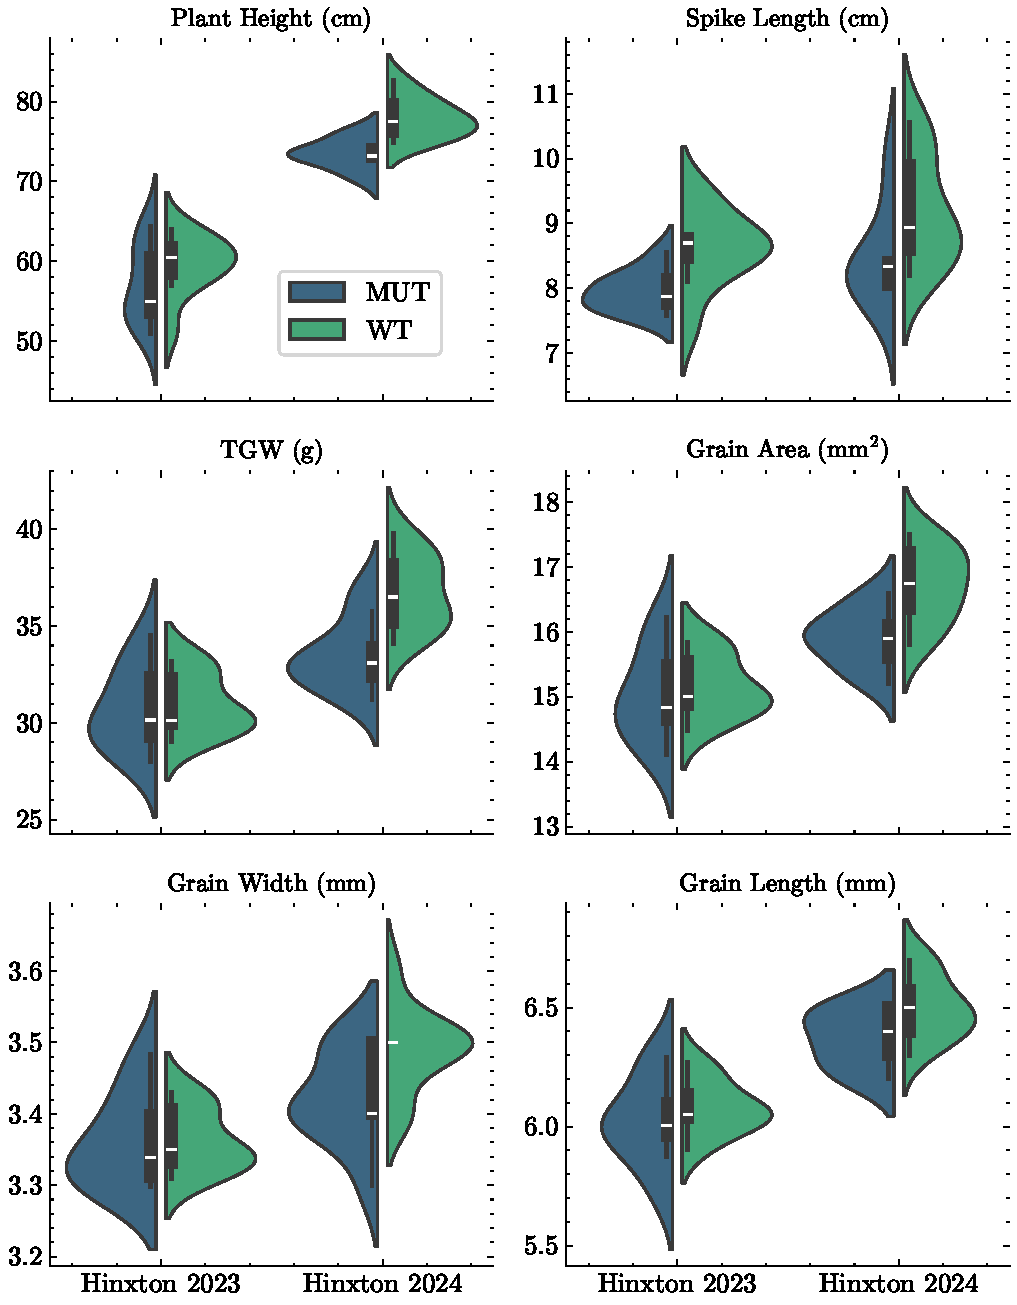
\includegraphics[width=\textwidth]{Hinx 23 24 Combined Plot.pdf}
	\caption{Physiological traits of the \textit{srh1} mutant and wild-type plants
		in 2023 and 2024 Hinxton Nurseries.}
	\label{Hinx_23_24_combined}
\end{figure}

\subsection{Isotope Discrimination}
From flag leaves sampled on 27/6/2024, mean leaf nitrogen \% (4.03$\pm$0.36)\%
in the \textit{srh1} mutant was similar to that of the wild-type (4.23$\pm$0.29)\%. $\delta$15N and
$\delta$13C values in the mutant also closely resembled those of the wild-type,
with mean $\delta$15N values of 2.75$\pm$0.87 for the \textit{srh1} mutant
and 2.73$\pm$1.3 for the wild-type. Mean $\delta$13C values were -27.4$\pm$0.98
for the mutant and -27.5$\pm$0.7 for the wild-type. Mean flag leaf carbon \%
was 41.2$\pm$0.92 in the mutant and 42.1$\pm$0.75 in the wild-type.

Variation in flag leaf N\% was the significant between technical replicates
(p \textless0.05) across both genotypes. Flag leaf carbon \% was significantly
different (p\textless0.05) between the \textit{srh1} mutant and wild-type, with the
mutant displaying a lower level of carbon in dried flag leaves compared to
the wild-type (Figure \ref{isotope_combined}, Table \ref{isotope_statistics}).
No significnat differences were observed between the genotypes across N\%,
$\delta$15N and $\delta$13C.

\begin{figure}[ht]
	\centering
	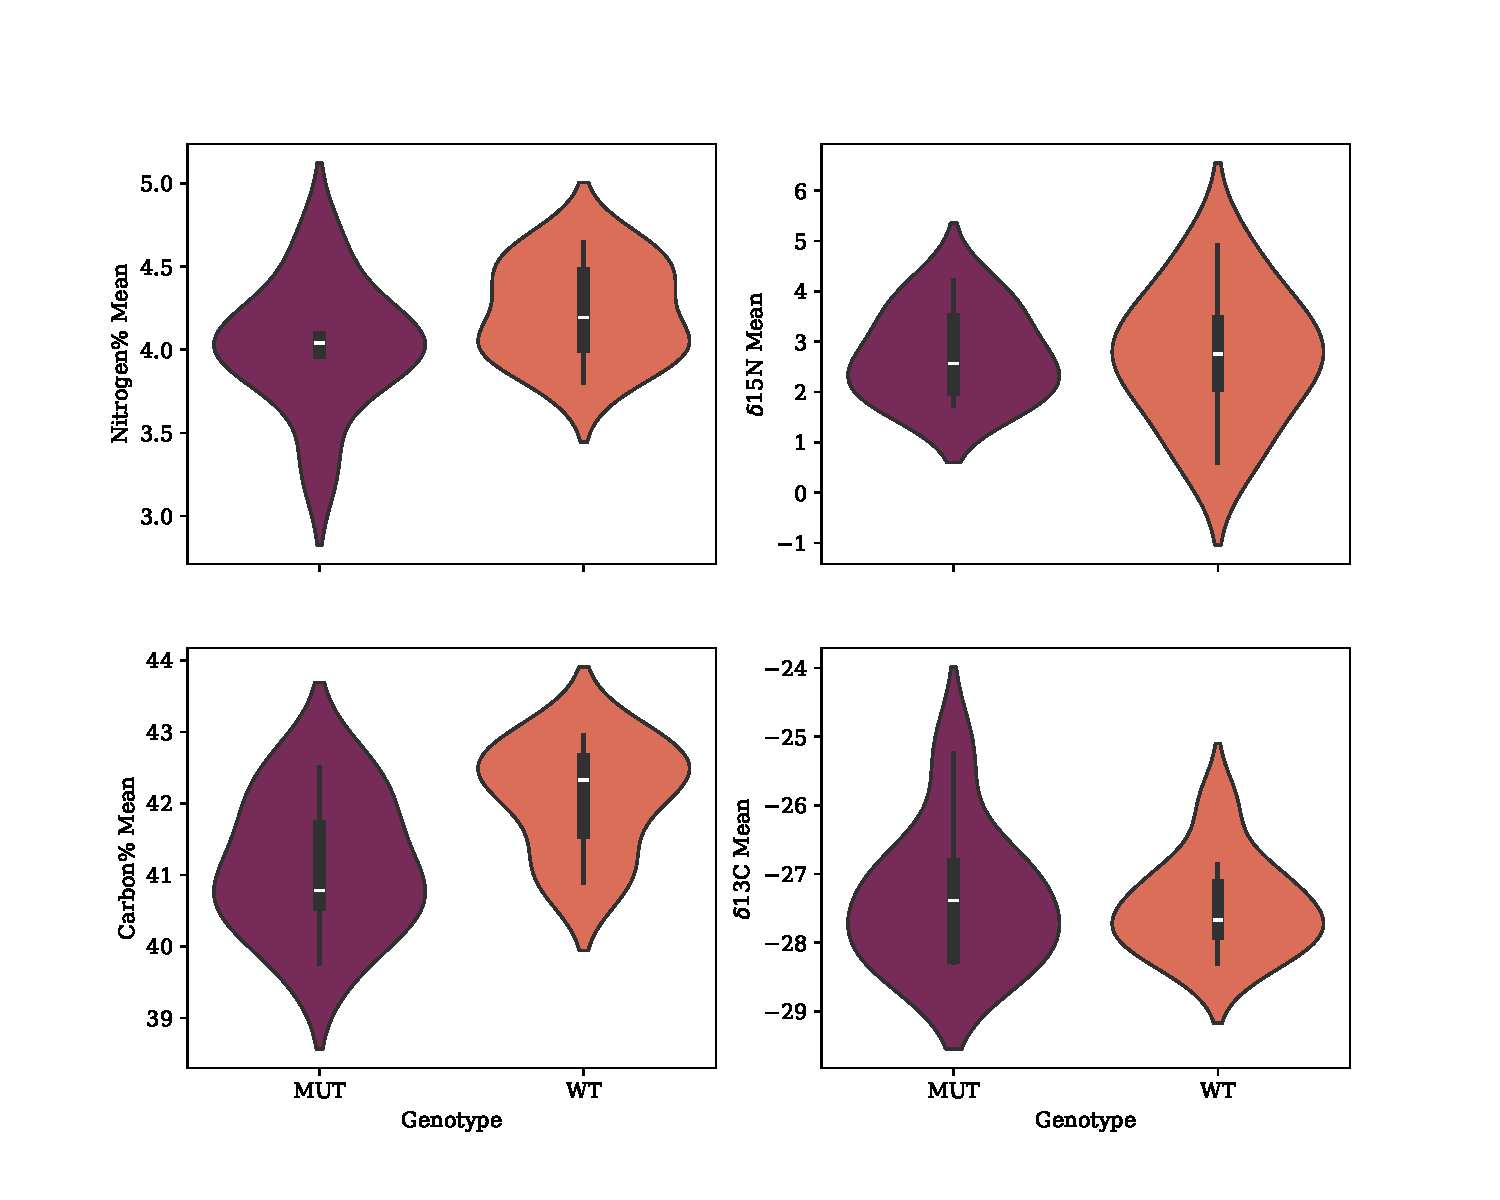
\includegraphics[width=\textwidth]{isotope.pdf}
	\caption{Isotope discrimination from flag leaf discs (harvested 27/6/24)
		of the \textit{srh1} mutant and wild-type plants grown in the 2024 nursery
		trial, measured via mass spectrometry.}
	\label{isotope_combined}
\end{figure}

\begin{table}[ht]
	\centering
	\caption{Summary statistics from flag leaf isotope discrimination}
	\label{isotope_statistics}
	\begin{adjustbox}
		{width=\textwidth}
		\begin{tabular}{@{}cllllllll@{}}
			\toprule \multicolumn{1}{l}{}         & \textbf{}     & \textbf{Sum Sq} & \textbf{Mean Sq} & \textbf{NumDF} & \textbf{DenDF} & \textbf{F value} & \textbf{Pr(\textgreater{}F)} &       \\
			\midrule \multirow{2}{*}{Nitrogen\%}  & Rep           & 0.06044         & 0.06044          & 1              & 37             & 4.7991           & 0.03485                      & *     \\
			                                      & Genotype      & 0.02339         & 0.02339          &  1              & 17             & 1.8572           & 0.19073                      &       \\
			\midrule \multirow{2}{*}{$\delta$15N} & Rep           & 0.04705         & 0.04705          & 1              & 37             & 1.7605           & 0.19269                      &       \\
			                                      & Genotype      & 0.00004         & 0.00004          & 1              & 17             & 0.0014           & 0.97099                      &       \\
			\midrule \multirow{2}{*}{Carbon\%}    & Rep           & 0.00609         & 0.00609          & 1              & 37             & 0.0198           & 0.88888                      &       \\
			                                      & Genotype      & 1.83507         & 1.83507          & 1              & 17             & 5.9667           & 0.02579                      & *     \\
			\midrule \multirow{2}{*}{$\delta$13C} & Rep           & 0.03384         & 0.03384          & 1              & 37             & 2.2593           & 0.1413                       &       \\
			                                      & Genotype      & 0.00104         & 0.00104          & 1              & 17             & 0.0692           & 0.79568                      &       \\
			\multicolumn{1}{l}{}                  & ---           &                 &                  &                &                &                  &                              &       \\
			\multicolumn{1}{l}{}                  & Signif. codes & : 0 '*          & **' 0.00         & 1 '**'         & 0.01           & '*' 0.05         & '.' 0.1                      & ' ' 1 \\
			\bottomrule
		\end{tabular}
	\end{adjustbox}
\end{table}

\subsection{Physiology Prediction}
\subsubsection{Variation in Spectral Reflectance}
Across all wavelengths (300$nm$-2500$nm$), significant variation was observed in
mean spectral reflectance between the \textit{srh1} mutant and wild-type
plants across the 6 timepoints. Mean reflectance at 7/8/2024 (start of
senescence) was most significantly different from the spectral curves of the
other 5 time points, with the greatest differences observed between the
wavelengths of 350$nm$-700$nm$, 770$nm$-1360$nm$, 1400$nm$-1850$nm$ and 1880$nm$-2500$nm$ (Figure
\ref{mean_spectral_reflctance}).
\begin{figure}[ht]
	\centering
	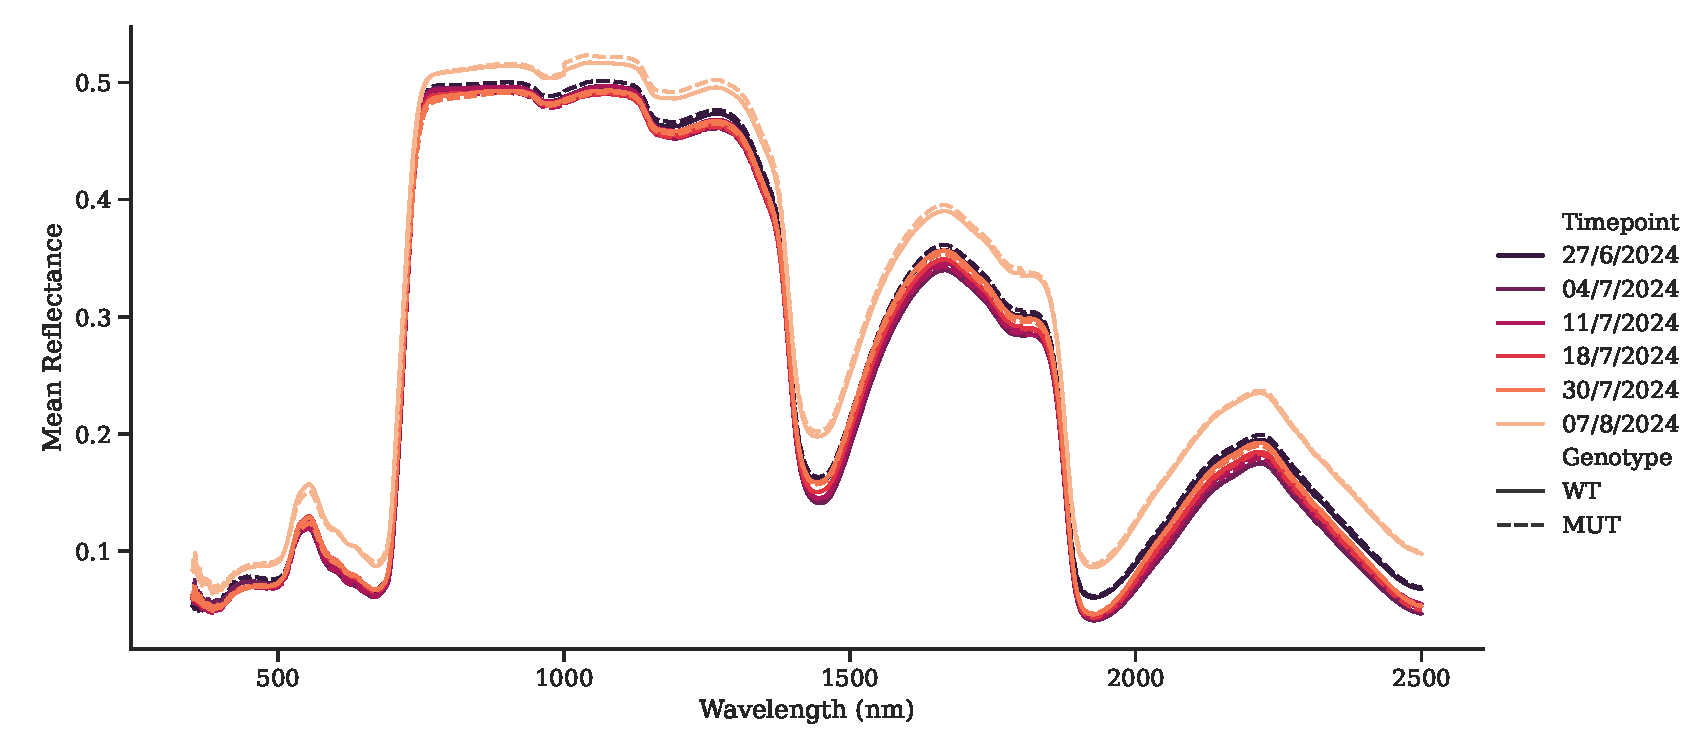
\includegraphics[width=\textwidth]{Mean Spectra Timepoint.pdf}
	\caption{Mean spectral reflectance from flag leaves of the \textit{srh1}
		mutant and wild-type grown in the field in 2024. Colours represent mean reflctance
		from different measurement time points; solid lines indicate \textit{srh1},
		dashed lines indicate wild-type.}
	\label{mean_spectral_reflctance}
\end{figure}

Within each timepoint, spectral reflectance also varied significantly within
each genotype. For example, at 17/8/2024, variation in spectral reflectance in
the wild-type plants ranged from a minimum value of 0.426 to a maximum value
of 0.529 at 1000$nm$ (Figure \ref{example_mut_trace}). Median and mean values
were 0.484 and 0.483 respectively with a standard error of 0.018.

\begin{figure}[ht]
	\centering
	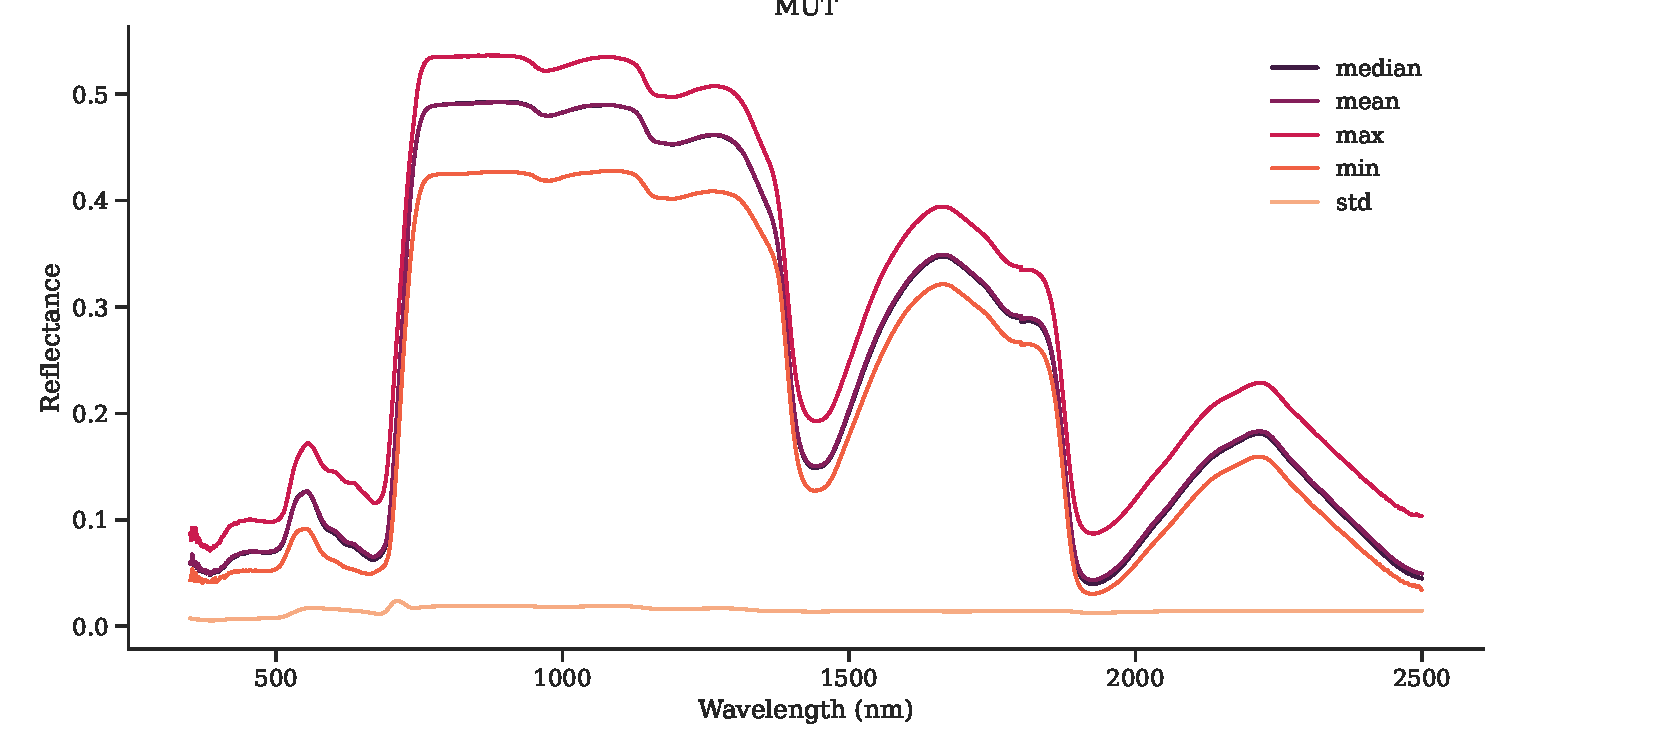
\includegraphics[width=\textwidth]{Mut Trace.pdf}
	\caption{Variation in spectral reflectance in wild-type leaves at 18/7/24
		(Flowering/Anthesis).}
	\label{example_mut_trace}
\end{figure}

\begin{figure}[ht]
	\centering
	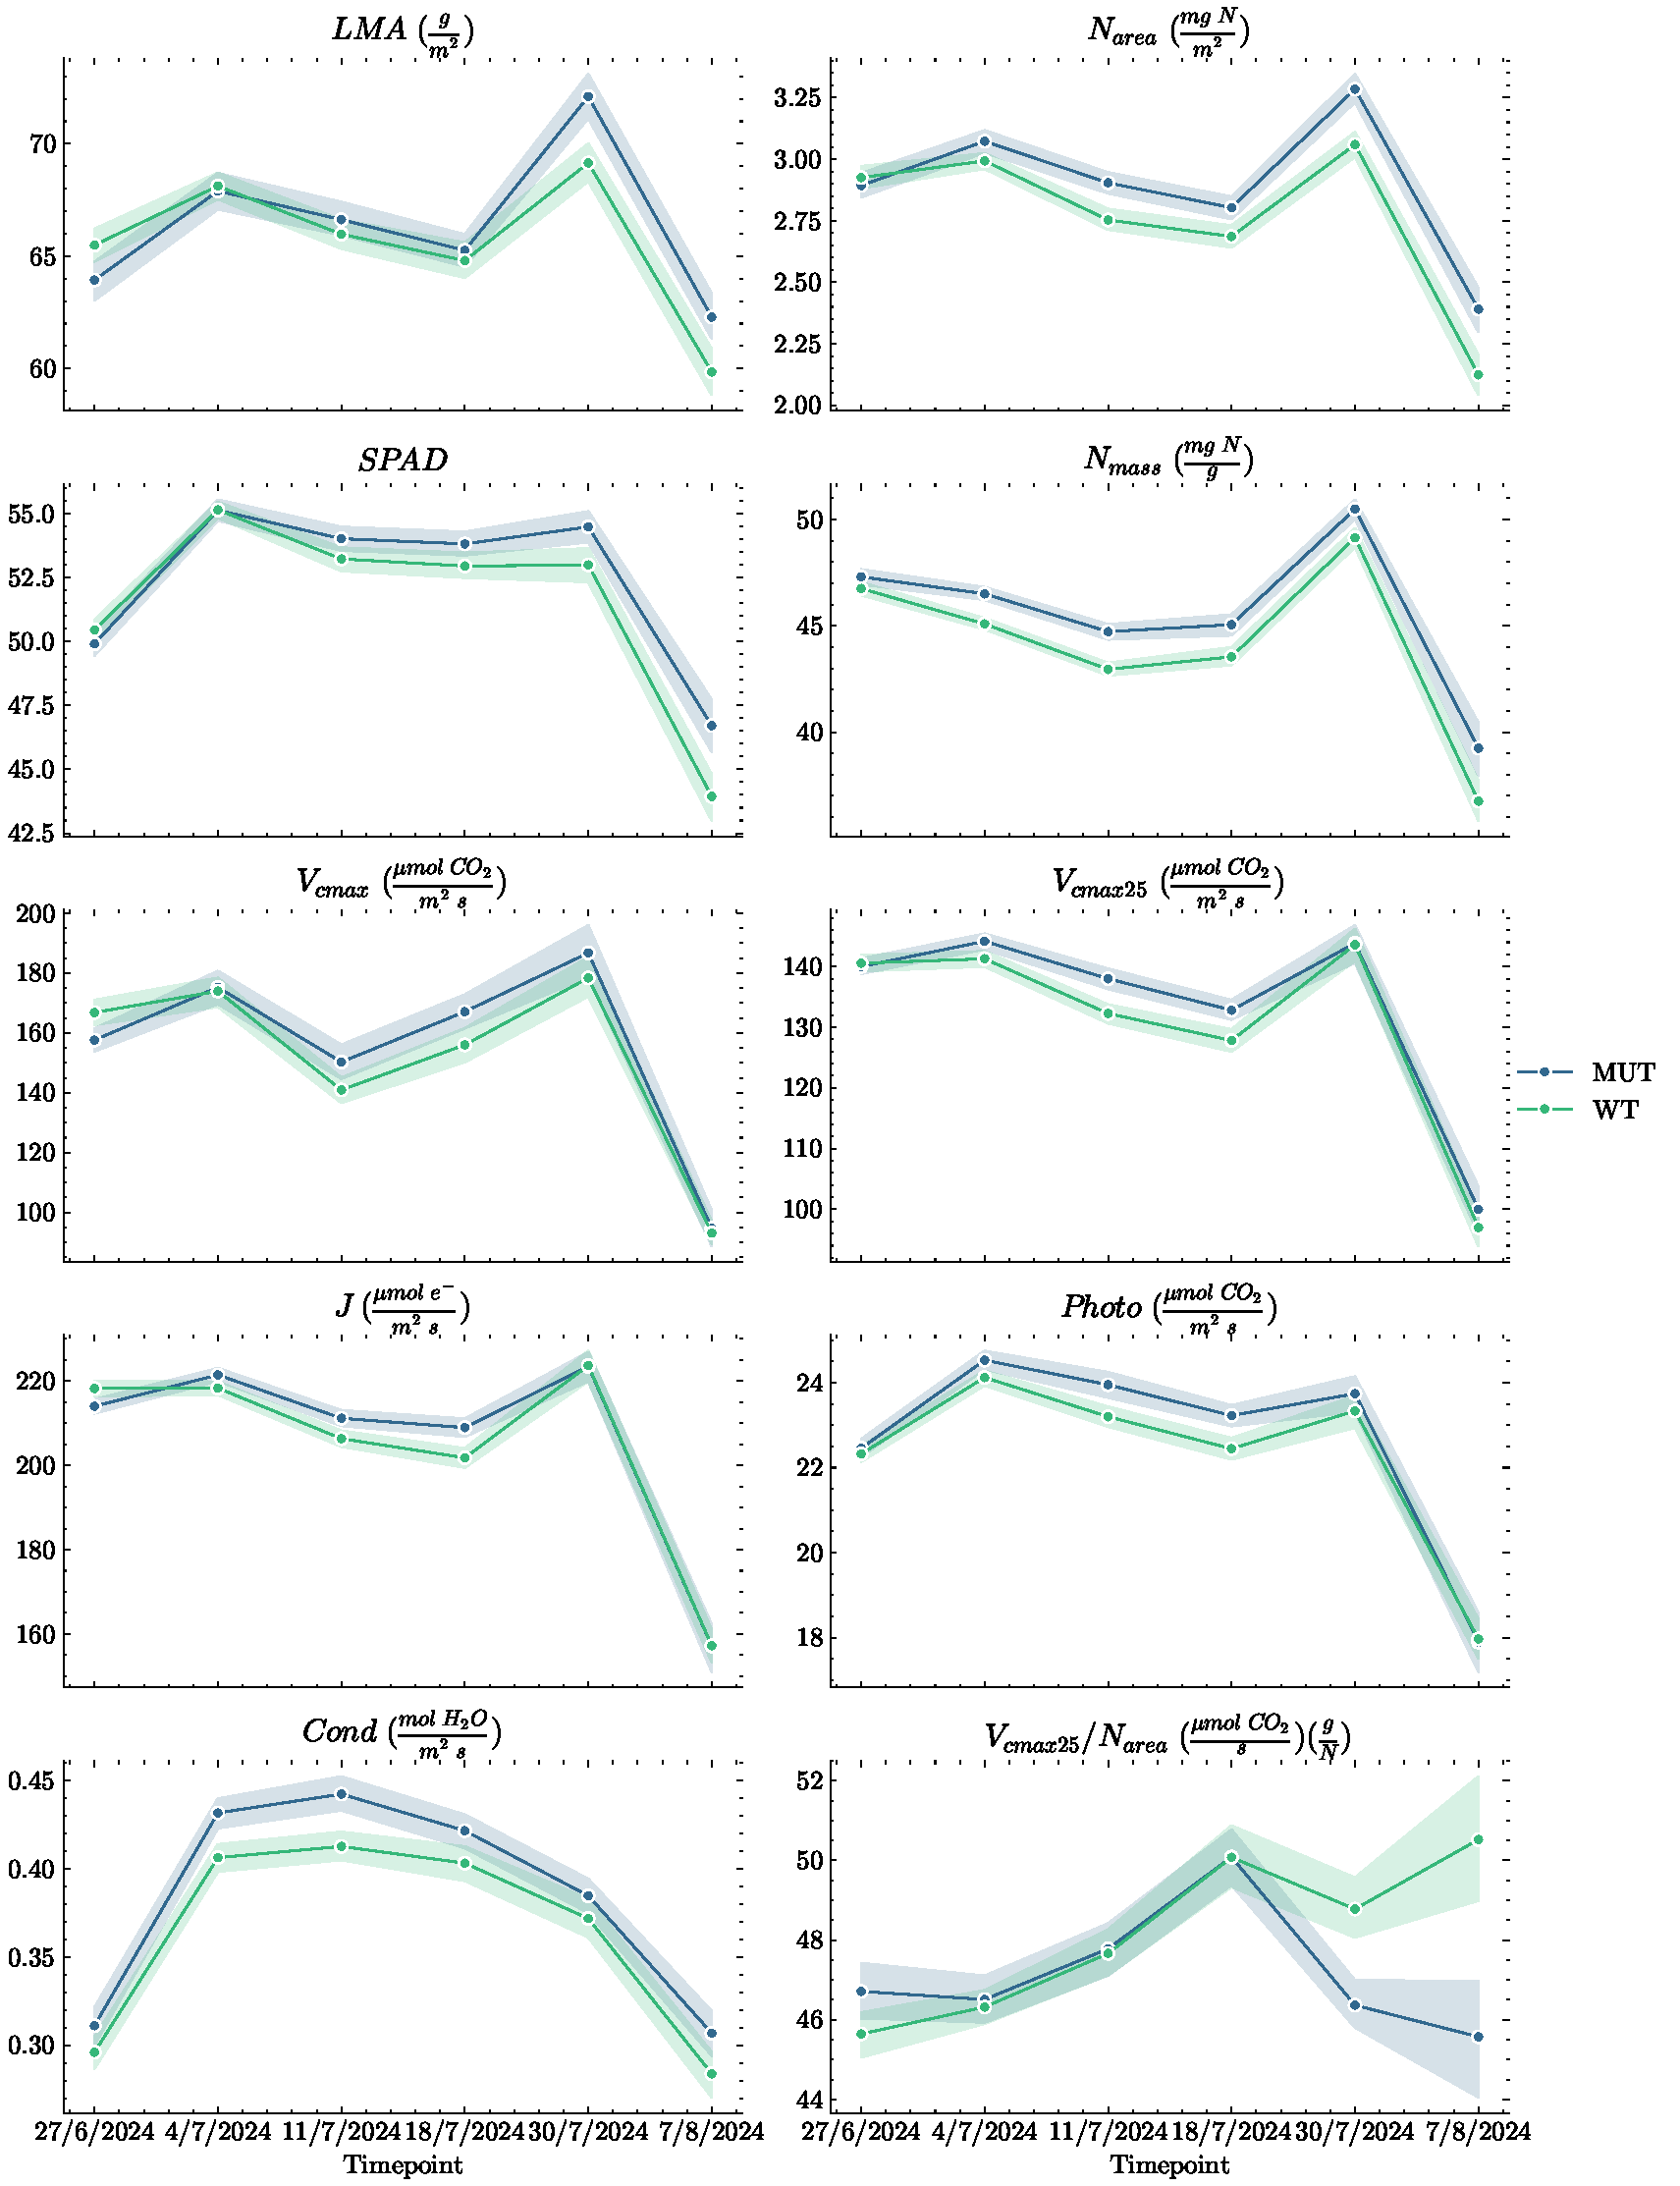
\includegraphics[width=0.9\textwidth, height=0.9\textheight]{
		Timeseries.pdf
	}
	\caption{Physiology traits predicted using Wheat Physiology Predictor (\cite{furbank_wheat_2021})
		from raw spectral reflectance data. Solid lines illustrate mean values across
		all plots for each gneotype, bands indicate range of data.}
	\label{timeseries_field_spec}
\end{figure}

\begin{table}[ht]
	\centering
	\caption{Summary statistics for predicted traits from spectral
		reflectance data}
	\label{field_spec_table}
	\begin{adjustbox}
		{width=\textwidth}
		\begin{tabular}{@{}cllllllll@{}}
			\toprule                                          &                    & \textbf{Sum Sq} & \textbf{Mean Sq} & \textbf{NumDF} & \textbf{DenDF} & \textbf{F value} & \textbf{Pr(\textgreater{}F)} &     \\
			\midrule \multirow{3}{*}{LMA}                     & Genotype           & 9               & 9.5              & 1              & 17             & 1.9211           & 0.183646                     &     \\
			                                                  & Timepoint          & 975             & 195              & 5              & 85             & 39.4359          & \textless 2.2e-16            & *** \\
			                                                  & Genotype:Timepoint & 70              & 14.1             & 5              & 85             & 2.851            & 0.019853                     & *   \\
			\midrule \multirow{3}{*}{N$_{area}$}              & Genotype           & 0               & 0.4              & 1              & 17             & 12.3942          & 0.002625                     & **  \\
			                                                  & Timepoint          & 10              & 1.9              & 5              & 85             & 65.6896          & \textless 2.2e-16            & *** \\
			                                                  & Genotype:Timepoint & 0               & 0                & 5              & 85             & 1.6759           & 0.149182                     &     \\
			\midrule \multirow{3}{*}{SPAD}                    & Genotype           & 19              & 18.8             & 1              & 17             & 5.2994           & 0.034247                     & *   \\
			                                                  & Timepoint          & 1257            & 251.4            & 5              & 85             & 70.9054          & \textless 2.2e-16            & *** \\
			                                                  & Genotype:Timepoint & 29              & 5.9              & 5              & 85             & 1.6518           & 0.15518                      &     \\
			\midrule \multirow{3}{*}{N$_{mass}$}              & Genotype           & 34              & 34.1             & 1              & 17             & 11.2546          & 0.003758                     & **  \\
			                                                  & Timepoint          & 1566            & 313.3            & 5              & 85             & 103.2761         & \textless 2.2e-16            & *** \\
			                                                  & Genotype:Timepoint & 7               & 1.3              & 5              & 85             & 0.4388           & 0.820228                     &     \\
			\midrule \multirow{3}{*}{$V_{cmax}$}              & Genotype           & 241             & 241.1            & 1              & 17             & 1.3253           & 0.265583                     &     \\
			                                                  & Timepoint          & 98756           & 19751.2          & 5              & 85             & 108.5845         & \textless 2.2e-16            & *** \\
			                                                  & Genotype:Timepoint & 1384            & 276.7            & 5              & 85             & 1.5214           & 0.19174                      &     \\
			\midrule \multirow{3}{*}{$V_{cmax25}$}            & Genotype           & 122             & 122              & 1              & 17             & 3.3062           & 0.086685                     & .   \\
			                                                  & Timepoint          & 28865           & 5772.9           & 5              & 85             & 156.4416         & \textless 2.2e-16            & *** \\
			                                                  & Genotype:Timepoint & 163             & 32.6             & 5              & 85             & 0.8839           & 0.49563                      &     \\
			\midrule \multirow{3}{*}{J}                       & Genotype           & 37              & 37.3             & 1              & 17             & 0.5287           & 0.477066                     &     \\
			                                                  & Timepoint          & 59094           & 11818.8          & 5              & 85             & 167.6234         & \textless 2.2e-16            & *** \\
			                                                  & Genotype:Timepoint & 467             & 93.5             & 5              & 85             & 1.3259           & 0.260994                     &     \\
			\midrule \multirow{3}{*}{Photo}                   & Genotype           & 2               & 2.3              & 1              & 17             & 2.2144           & 0.155039                     &     \\
			                                                  & Timepoint          & 525             & 105.1            & 5              & 85             & 100.984          & \textless 2.2e-16            & *** \\
			                                                  & Genotype:Timepoint & 5               & 1                & 5              & 85             & 0.9334           & 0.463637                     &     \\
			\midrule \multirow{3}{*}{Cond}                    & Genotype           & 0               & 0                & 1              & 102            & 16.0437          & 0.000118                     & *** \\
			                                                  & Timepoint          & 0               & 0.1              & 5              & 102            & 88.4021          & \textless 2.2e-16            & *** \\
			                                                  & Genotype:Timepoint & 0               & 0                & 5              & 102            & 0.2263           & 0.950356                     &     \\
			\midrule \multirow{3}{*}{$V_{cmax25}$/N$_{area}$} & Genotype           & 22              & 22               & 1              & 17             & 3.484            & 0.079312                     & .   \\
			                                                  & Timepoint          & 186             & 37.2             & 5              & 85             & 5.879            & 0.000103                     & *** \\
			                                                  & Genotype:Timepoint & 140             & 28               & 5              & 85             & 4.4251           & 0.001248                     & **  \\
			                                                  & ---                &                 &                  &                &                &                  &                              &     \\
			                                                  & Signif. codes:     & '***' 0.001     & '**' 0.01        & 1              & '*' 0.05 '     & .' 0.1 '         & ' 1                          &     \\
			\bottomrule
		\end{tabular}
	\end{adjustbox}
\end{table}

\subsubsection{Spectra QC}

\begin{figure}[H]
	\centering
	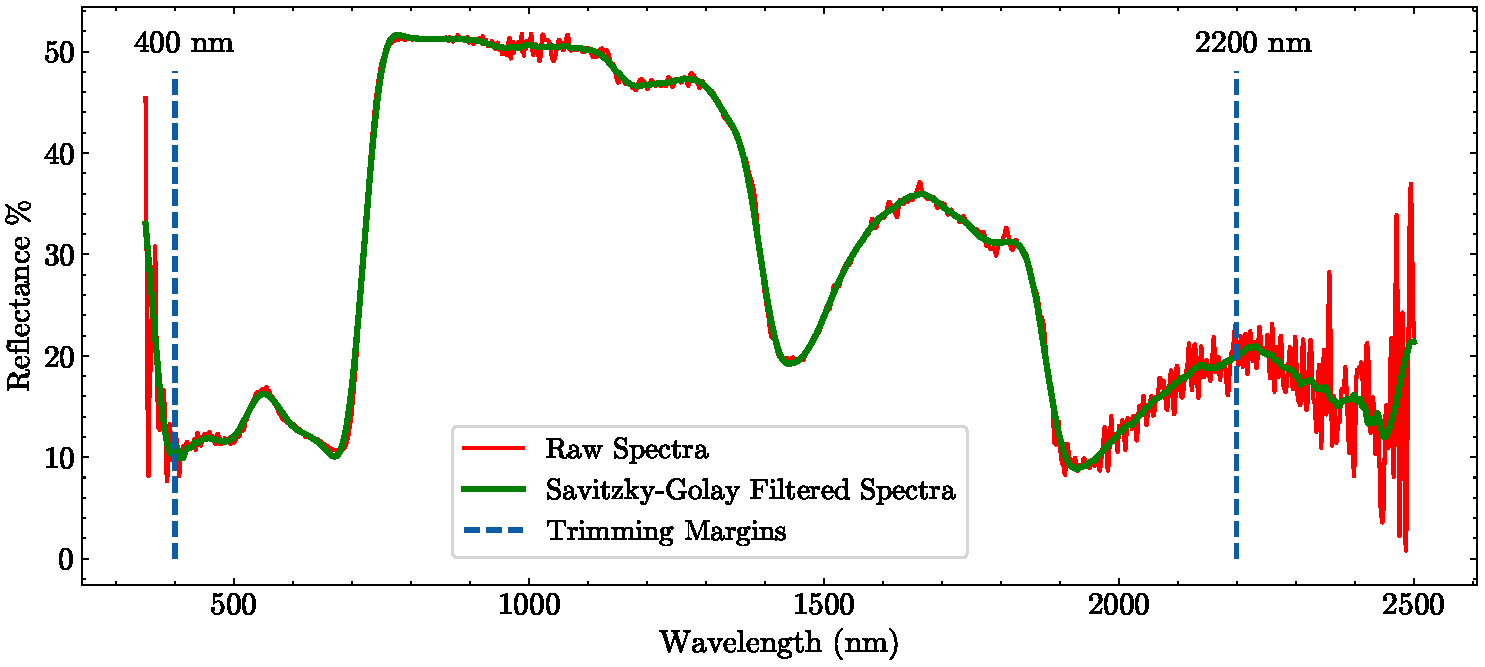
\includegraphics[width=\textwidth]{psr_spectra_qc.pdf}
	\caption{Example trace illustrating QC procedure for spectra obtained via the PSR+3500. Raw spectra in red, Savitzky-Golay filtered spectra in green with a window length of 100, polyorder of 2. Vertical blue dashed lines illustrate regions discarded post filtering. Wavelengths $\leq$ 400nm and $\geq$ 2200nm were discarded prior to trait prediction. }
	\label{psr_spectra_qc}
\end{figure}










\subsubsection{Predicted Traits}
All 10 predicted traits (Figure \ref{timeseries_field_spec}) varied significantly
(p \textless 0.001) between measurement timepoints (Table \ref{field_spec_table}).
Aside from V$_{cmax25}$/N$_{area}$, all other traits experienced a large drop-off
in mean values at 7/8/2024 relative to mean values from the other 5 timepoints.

A significant interaction betwen Genotype and Timepoint was found in Leaf Mass
Area (LMA) (p \textless 0.05) and V$_{cmax25}$/N$_{area}$ (p \textless 0.01) (Table
\ref{field_spec_table}). The greatest difference in LMA between \textit{srh1}
and wild-type was during 30/7/24, where mean LMA value for the \textit{srh1}
mutant was 72.1$\pm$2.5 g/m$^{2}$ compared to 69.1$\pm$1.8 g/m$^{2}$ in the wild-type.
At 7/8/24, the mean V$_{cmax25}$/N$_{area}$ was greater in the wild-type (50.7$\pm$4.7
$\mu$mol CO2 s$^{-1}$(g N$^{-1}$)) than \textit{srh1} (45.2$\pm$5 $\mu$mol
CO2 s$^{-1}$(g N$^{-1}$)) (Figure \ref{timeseries_field_spec}).

Genotype (\textit{srh1} and wild-type) had a significant effect on LMA (p \textless
0.05), Leaf nitrogen area (N$_{area}$) (p \textless 0.01), leaf nitrogen mass (N$_{mass}$)
(p \textless 0.01), SPAD (Soil Plant Analysis Development - a surrogate for chlorophyll
content) (p \textless 0.05) and stomatal conductance (Cond) (p \textless 0.001) (Table \ref{field_spec_table}).

Genotype did not have a significant effect on V$_{cmax}$, V$_{cmax25}$, J (rate
of electron transport) and Photo (rate of CO$_{2}$ fixation per unit area).

\subsubsection{Relationships Between Predicted Traits}

LMA exhibited strong positive correlation with $N_{area}$ ($R^{2}$ = 0.82) and SPAD ($R^{2}$ = 0.77). $N_{area}$ was positively correlated with $N_{mass}$ ($R^{2}$ = 0.82), although this correlation was much weaker in measurements taken during the grain forming stage (30/7/2024) ($R^{2}$ = 0.28 for \textit{srh1} and $R^{2}$ = 0.30 for wild-type) compared to measurements during start of senescence (7/8/2024) ($R^{2}$ = 0.74 for \textit{srh1}, $R^{2}$ = 0.79 for wild-type) (Figure \ref{correlation_matrix}).

J and $V_{cmax25}$ were the two most strongly correlated traits ($R^{2}$ = 0.95), where the relationship between J and $V_{cmax25}$ was consistent between the \textit{srh1} mutant and wild-type, and at each timepoint. Measurements taken during the start of senescence (7/8/2024) displayed the strongest correlation between J and $V_{cmax25}$ ($R^{2}$ = 0.94 for \textit{srh1} and $R^{2}$ = 0.93 for wild-type) (Figure \ref{correlation_matrix}).

$V_{cmax25}/N_{area}$ was negatively correlated with LMA ($R^{2}$ = -0.6), $N_{area}$ ($R^{2}$ = -0.6) and SPAD ($R^{2}$ = -0.5) (Figure \ref{correlation_matrix}).





\begin{figure}[ht]
	\centering
	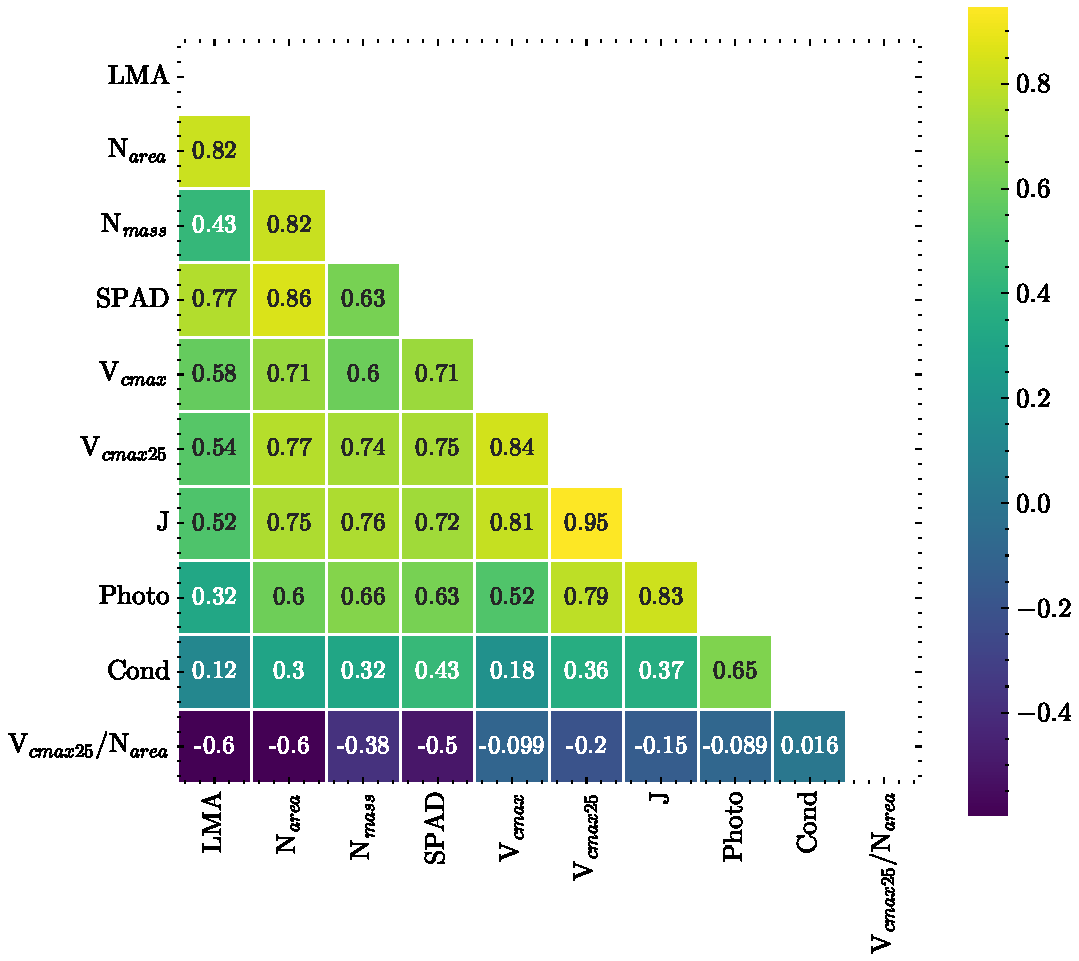
\includegraphics[width=\textwidth]{Correlation Matrix.pdf}
	\caption{Correlation matrix illustrating relationships between the ten predicted traits for both genotypes across all timepoints.}
	\label{correlation_matrix}
\end{figure}




\subsection{Field Scanalyzer}
\subsubsection{Plant Height}
Across the 9 timepoints performed by the laser scanner, mean height of the
\textit{srh1} mutant was consistently shorter than the wild-type. Initial
scans at 30/5/2024 indicated plant height in the mutant (14.2$\pm$3.45 $cm$) was
shorter than the wild-type (18.3$\pm$5.26 $cm$). The largest difference in plant
height between the genotypes occured during 19/7/2024 (Anthesis), where the
\textit{srh1} mutant was 4.81 $cm$ shorter than the wild-type. The rate of height
growth between each timepoint was relatively consistent between the \textit{srh1}
and wild-type.

Plant Height was statistically influenced by Genotype and Timepoint. Differences
in plant height between different timepoints (p \textless 0.001) are clearly reflected
in the steady increase in plant height across the growing season in both the
\textit{srh1} mutant and wild-type (Figure \ref{height}, Table
\ref{scanalyzer_table}). Genotype had a significant effect on plant height (p
\textless 0.05, Table \ref{scanalyzer_table}), where the \textit{srh1} mutant was consistently
shorter than the wild-type across all recorded timepoints (Figure
\ref{height}). No statistical difference in the growth rate of plant height
across both genotypes was detected (Table \ref{scanalyzer_table}).

\subsubsection{FVC}
FVC was measured from the RGB images across 17 timepoints from May\hyp{}Aug.
The mean FVC of the \textit{srh1} mutant plots were consistently lower than mean
FVC of wild-type plots. Mean FVC values progressed smoothly across
timepoints until reaching a maximum FVC value at 23/7/24, where mean FVC in the
wild-type was 0.32$\pm$0.06 compared to 0.23$\pm$0.06 in the \textit{srh1}
mutant. Subsequent drop-off in mean FVC occured in both the \textit{srh1}
mutant and wild-type from 23/7/24 to 12/8/24.

Timepoint had a significant effect on FVC, where FVC increased consistently
throughout the growth season up until 23/7/24, where FVC values subsequently
decreased at 12/8/24. Genotype was not found to significantly affect FVC,
and no differences in FVC growth rate were found (Table \ref{scanalyzer_table}).

\begin{table}[ht]
	\centering
	\caption{Summary statistics for plant height, height growth rate, FVC
		and FVC growth rate between the \textit{srh1} mutant and wild-type.}
	\label{scanalyzer_table}
	\begin{adjustbox}
		{width=\textwidth}
		\begin{tabular}{@{}cllllllll@{}}
			\toprule \multicolumn{1}{l}{\textbf{}}      &               & \textbf{SumSq} & \textbf{MeanSq} & \textbf{NumDF} & \textbf{DenDF} & \textbf{F value} & \textbf{Pr(\textgreater{}F)} &     \\
			\midrule \multirow{3}{*}{Plant Height}      & Generation    & 2              & 1.7             & 1              & 12             & 0.2766           & 0.6085                       &     \\
			                                            & Timepoint     & 45229          & 5653.7          & 8              & 120            & 912.2813         & \textless{}2e-16             & *** \\
			                                            & Genotype      & 32             & 31.8            & 1              & 12             & 5.1254           & 0.0429                       & *   \\
			\midrule \multirow{3}{*}{FVC}               & Generation    & 0.00003        & 0.000033        & 1              & 12             & 0.0455           & 0.83466                      &     \\
			                                            & Timepoint     & 1.84274        & 0.115171        & 16             & 240            & 158.9563         & \textless 2e-16              & *** \\
			                                            & Genotype      & 0.00273        & 0.002734        & 1              & 12             & 3.7728           & 0.07593                      & .   \\
			\midrule \multirow{4}{*}{Plant Height Rate} & Generation    & 0              & 0               & 1              &                & 0.0002           & 0.99                         &     \\
			                                            & Timepoint     & 49.424         & 6.1781          & 8              &                & 56.0903          & \textless{}2e-16             & *** \\
			                                            & Genotype      & 0.004          & 0.0045          & 1              &                & 0.0406           & 0.8406                       &     \\
			                                            & Residuals     & 14.649         & 0.1101          & 133            &                &                  &                              &     \\
			\midrule \multirow{4}{*}{FVC Rate}          & Generation    & 4.2E-06        & 4.19E-06        & 1              &                & 0.179            & 0.6726                       &     \\
			                                            & Timepoint     & 0.008223       & 0.000514        & 16             &                & 21.9806          & \textless{}2e-16             & *** \\
			                                            & Genotype      & 5.8E-06        & 5.76E-06        & 1              &                & 0.2464           & 0.62                         &     \\
			                                            & Residuals     & 0.005892       & 2.34E-05        & 252            &                &                  &                              &     \\
			\multicolumn{1}{l}{}                        & -             &                &                 &                &                &                  &                              &     \\
			\multicolumn{1}{l}{}                        & Signif.codes: & 0              & '***' 0.001     & '**' 0.01      & '*' 0.05       & '.' 0.1          & ' ' 1                        &     \\
			\bottomrule
		\end{tabular}
	\end{adjustbox}
\end{table}






\begin{figure}[ht]
	\centering
	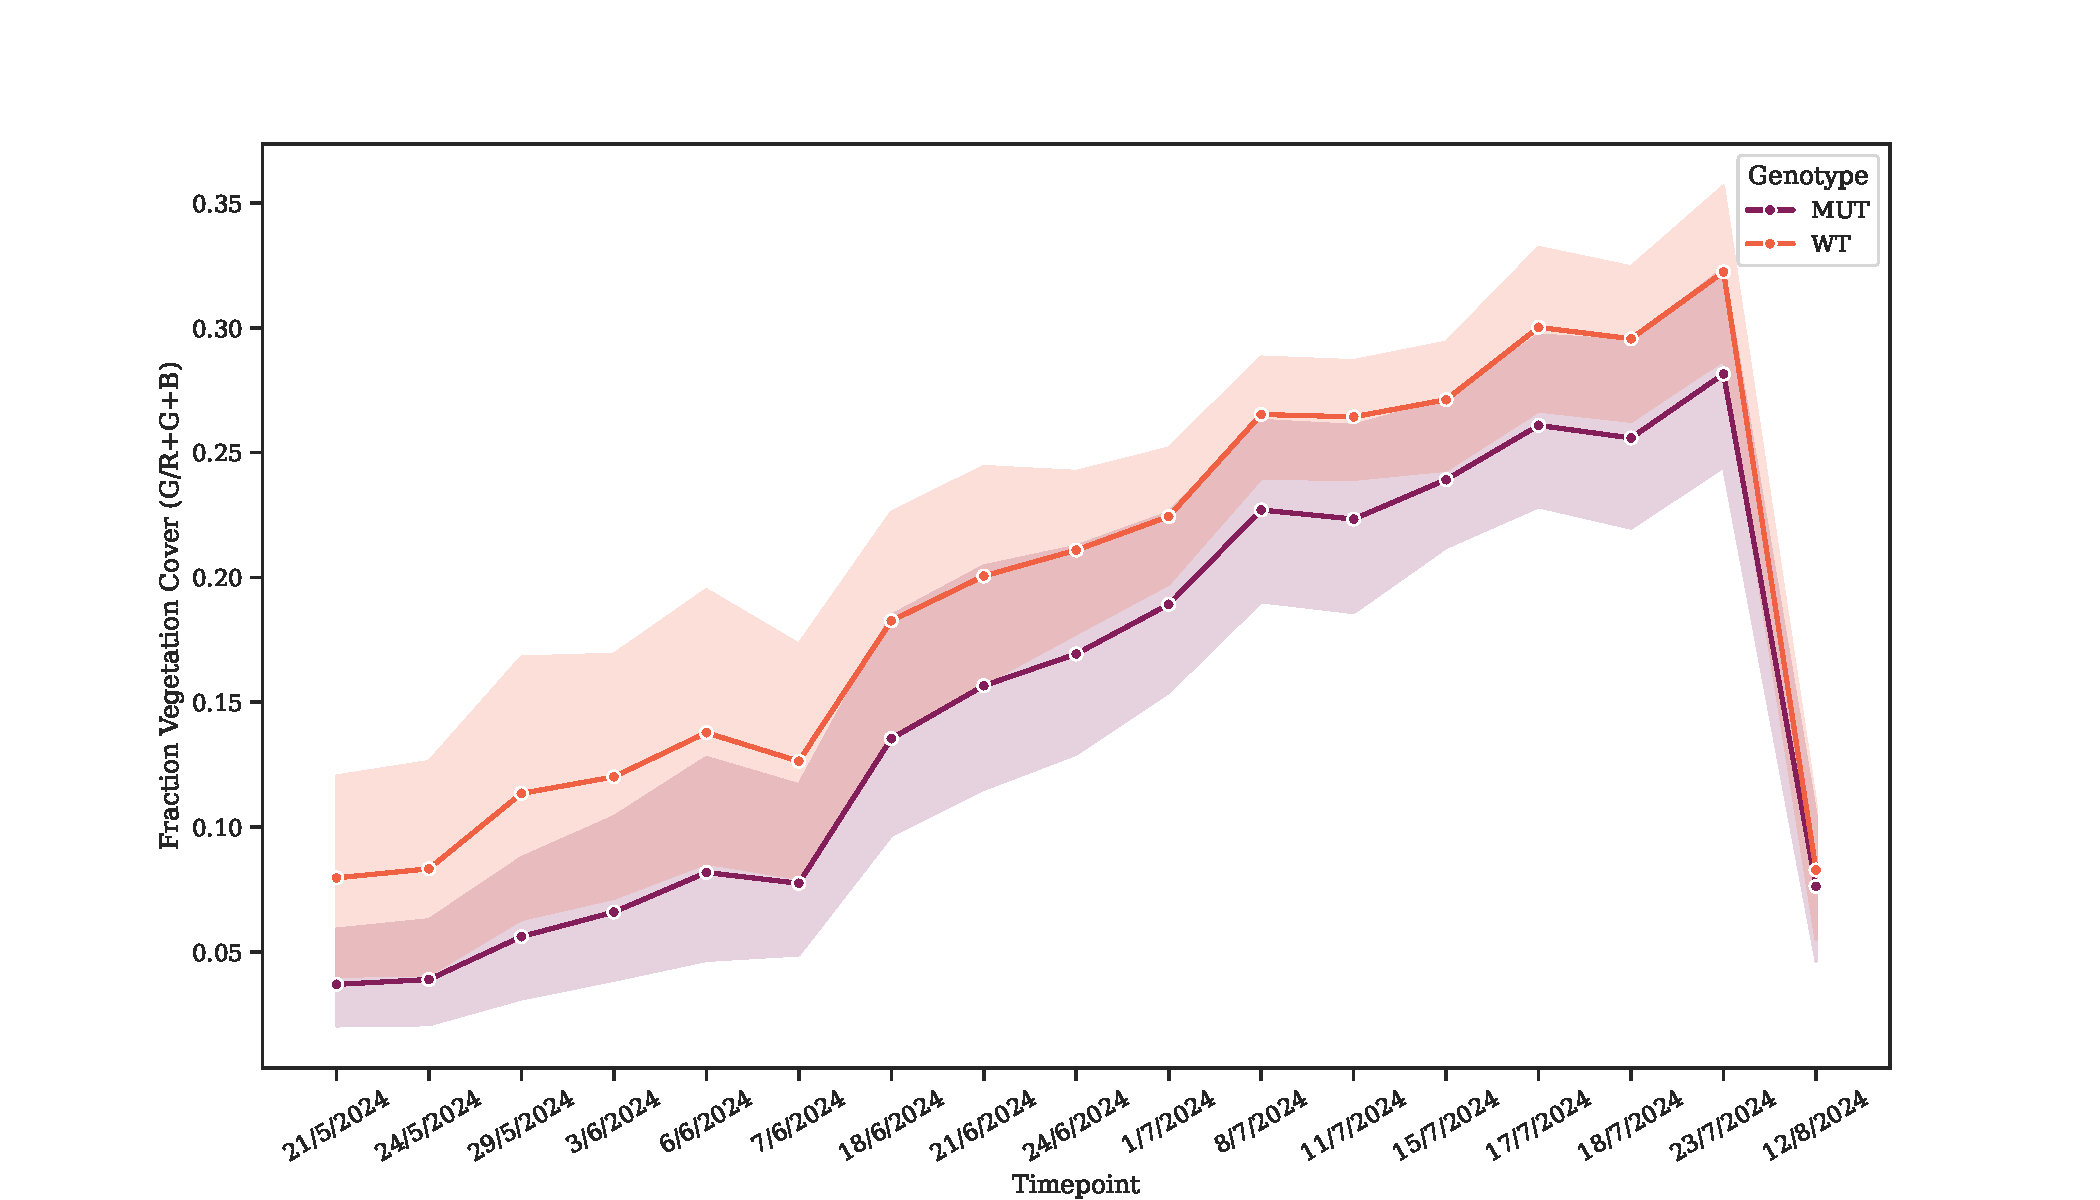
\includegraphics[width=\textwidth]{FVC.pdf}
	\caption{Fraction Vegetation Cover (FVC) in the \textit{srh1} mutant and
		wild-type from emergence till senescence, grown at Rothamstead Research
		in 2024. FVC was calculated from RGB images taken by the Field
		Scanalyzer. FVC is expressed as a ratio of green pixels to total pixels.
		Solid line illustrates mean FVC for each timepoint, bands illustrate range.}
	\label{fvc}
\end{figure}

\begin{figure}[ht]
	\centering
	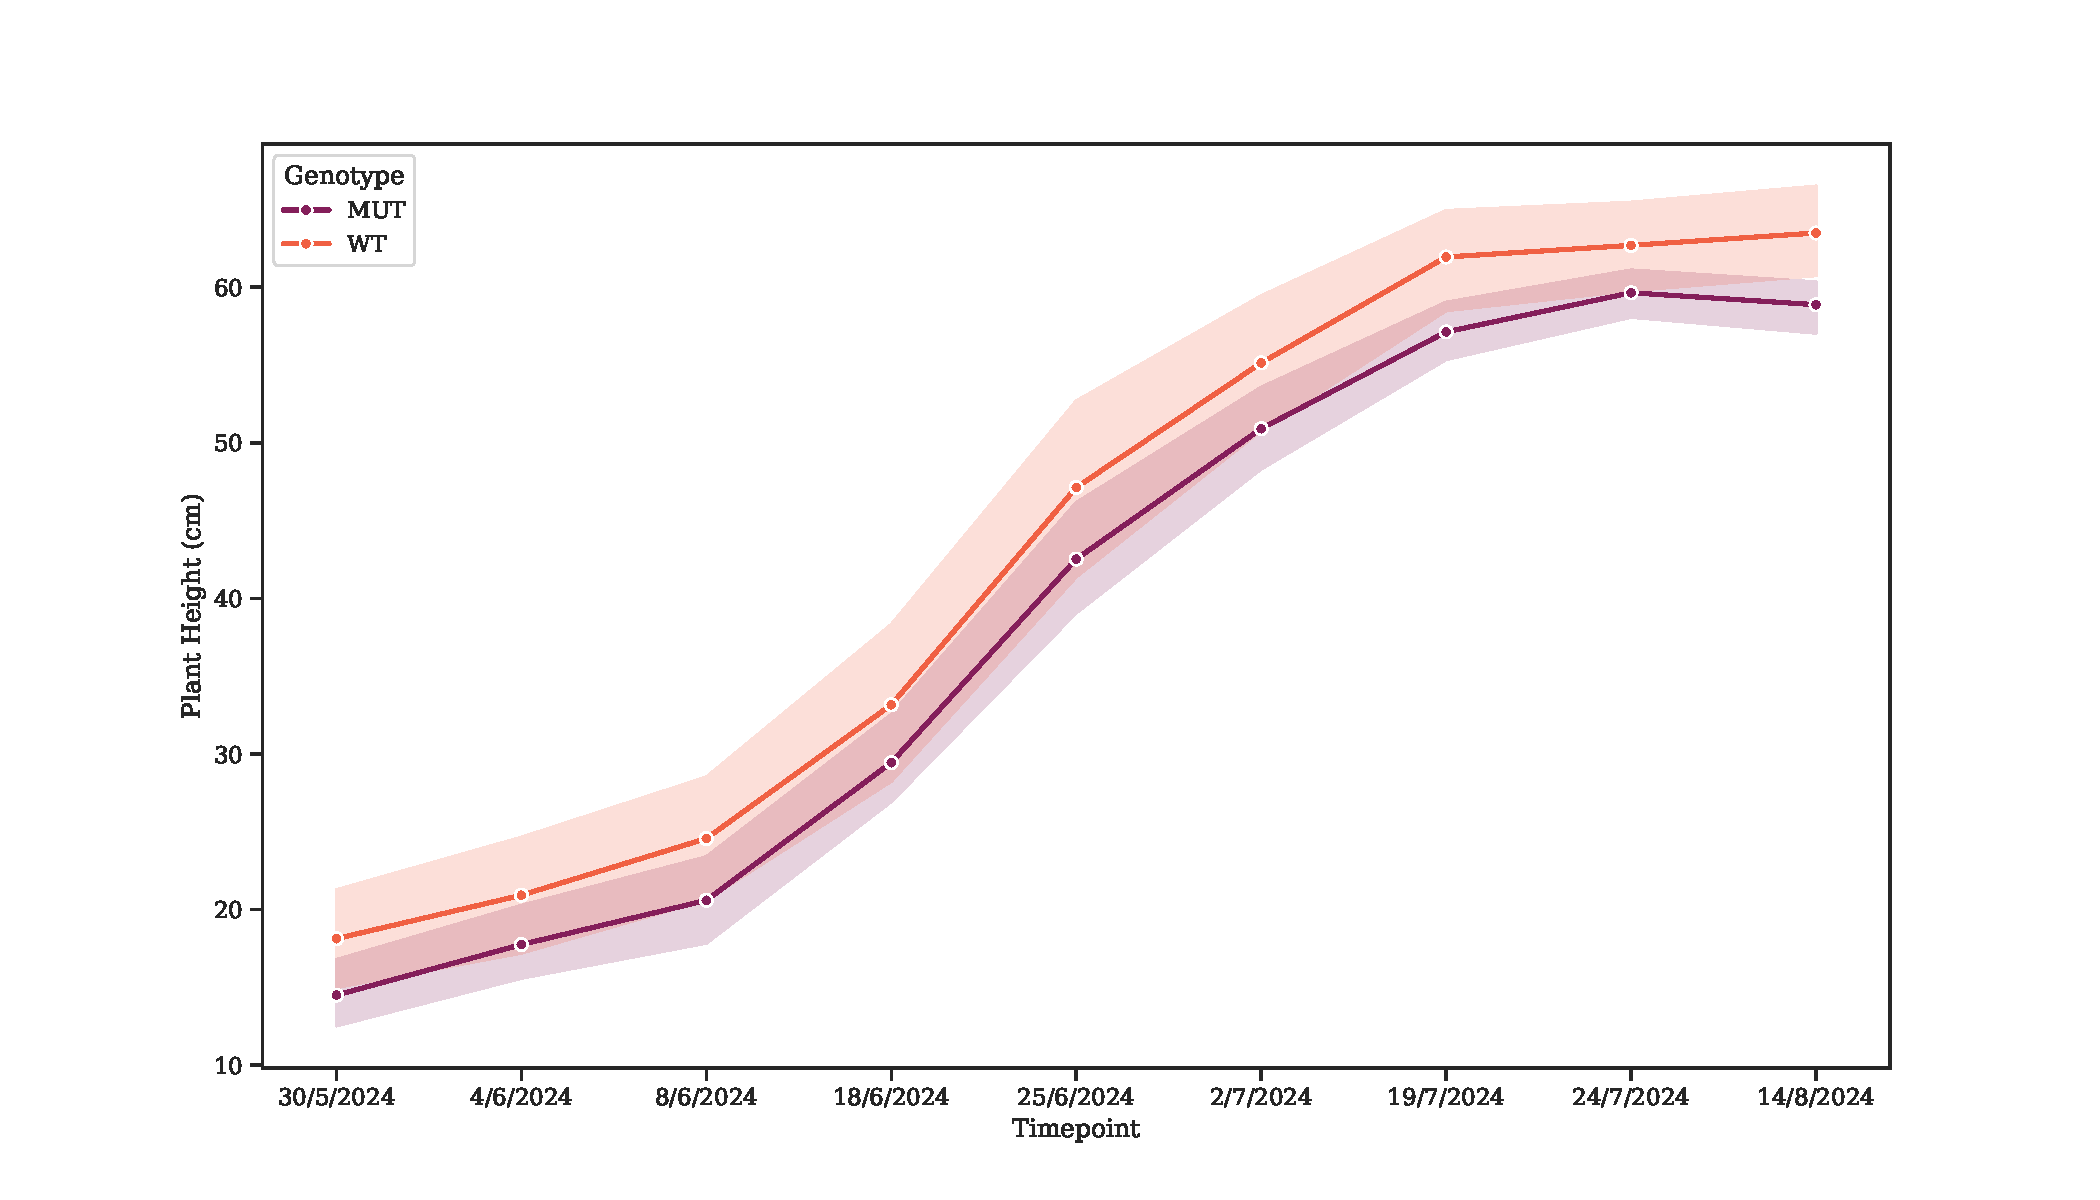
\includegraphics[width=\textwidth]{Height.pdf}
	\caption{Plant Height (cm) of the \textit{srh1} mutant and wild-type grown
		at Rothamstead Research in 2024. Plant Height was calculated from 3D point
		clouds of each plot via the laser scanner on the Field Scanalyzer. Solid
		line illustrates mean plant height for each timepoint, bands illustrate range.}
	\label{height}
\end{figure}


\section{Discussion}

\subsection{Root hairs influence a multitude of traits}







\subsection{FVC}
It is important to note that FVC does not directly account for differences
in growth rates etc. FVC is affected by emergence time, tiller number. However,
we have shown that there was no statistical difference in the growth rate of
both plant height and FVC between the \textit{srh1} mutant and wild-type overall,
and at each specific timepoint. Tiller number different? - pending...




\printbibliography


\end{document}

